\chapter{Implementation}
\label{chap:impl}

\section{System architecture}
\label{chap:impl:system-architecture}
  Biohadoop is a framework for running parallel algorithms on Apache Hadoop. It works according to the master - worker principle, where one master commands several workers. The master typically implements an algorithm, whose compute intense parts are executed by the workers in parallel.
  
  The framework relies on YARN (chapter \ref{chap:hadoop:yarn}) and provides features, that otherwise need to be implemented manually, such as:
  
  \begin{enumerate}
    \item support for running several algorithms in a single Biohadoop instance. This has the advantage that workers, and therefor resources, can be shared by the algorithms
    \item asynchronous communication between master and workers using a simple task system (section \ref{chap:impl:task-system})
    \item storage and load of arbitrary data to a file system (section \ref{chap:impl:persistence})
    \item support for the island model, a high level parallelization that can be used to improve the optimization performance of bio-inspired optimization techniques (section \ref{chap:impl:island-model})
    \item support by Apache Oozie through a custom action (section \ref{chap:impl:oozie}). This custom action can be used to start Biohadoop as a single instance, or to start several instances in parallel
  \end{enumerate}
  
  Every YARN application needs a client that submits the application to YARN. In Biohadoop, the client is implemented in the class \texttt{BiohadoopClient}. It is the main entrance point to run Biohadoop in a Hadoop environment and responsible to start the ApplicationMaster under the control of Hadoop.
  
  The ApplicationMaster's main class is \texttt{BiohadoopApplicationMaster}. In a local (development) environment, it acts as the main entrance point to run Biohadoop (more on how to run Biohadoop can be found in \ref{chap:usage:run}). The ApplicationMaster is responsible for the start of the configured workers in additional YARN containers, and as it is the master in the master - worker scheme, it executes the configured algorithms and communicates with the workers.
  
  The communication between the master and its workers is hidden from the algorithm (and therefor the user) by the task system. It provides a simple interface through the \texttt{TaskSubmitter} class. This interface can be used to submit work items, the so called tasks, to the task system, along with details of how the computation should be performed. The tasks are stored in a queue, the \texttt{TaskQueue}, until their result is known. Endpoints take the tasks and their configurations out of the queue and send them to waiting workers. The workers execute the configured computations on the tasks and return the results to the endpoints, that promote the results back to the \texttt{TaskQueue} and from there to the algorithms. Figure \ref{fig:architecture} gives a graphical representation of this concepts, more details about the task system can be found in section \ref{chap:impl:task-system}
  
  \begin{figure}[ht!]
    \centering
    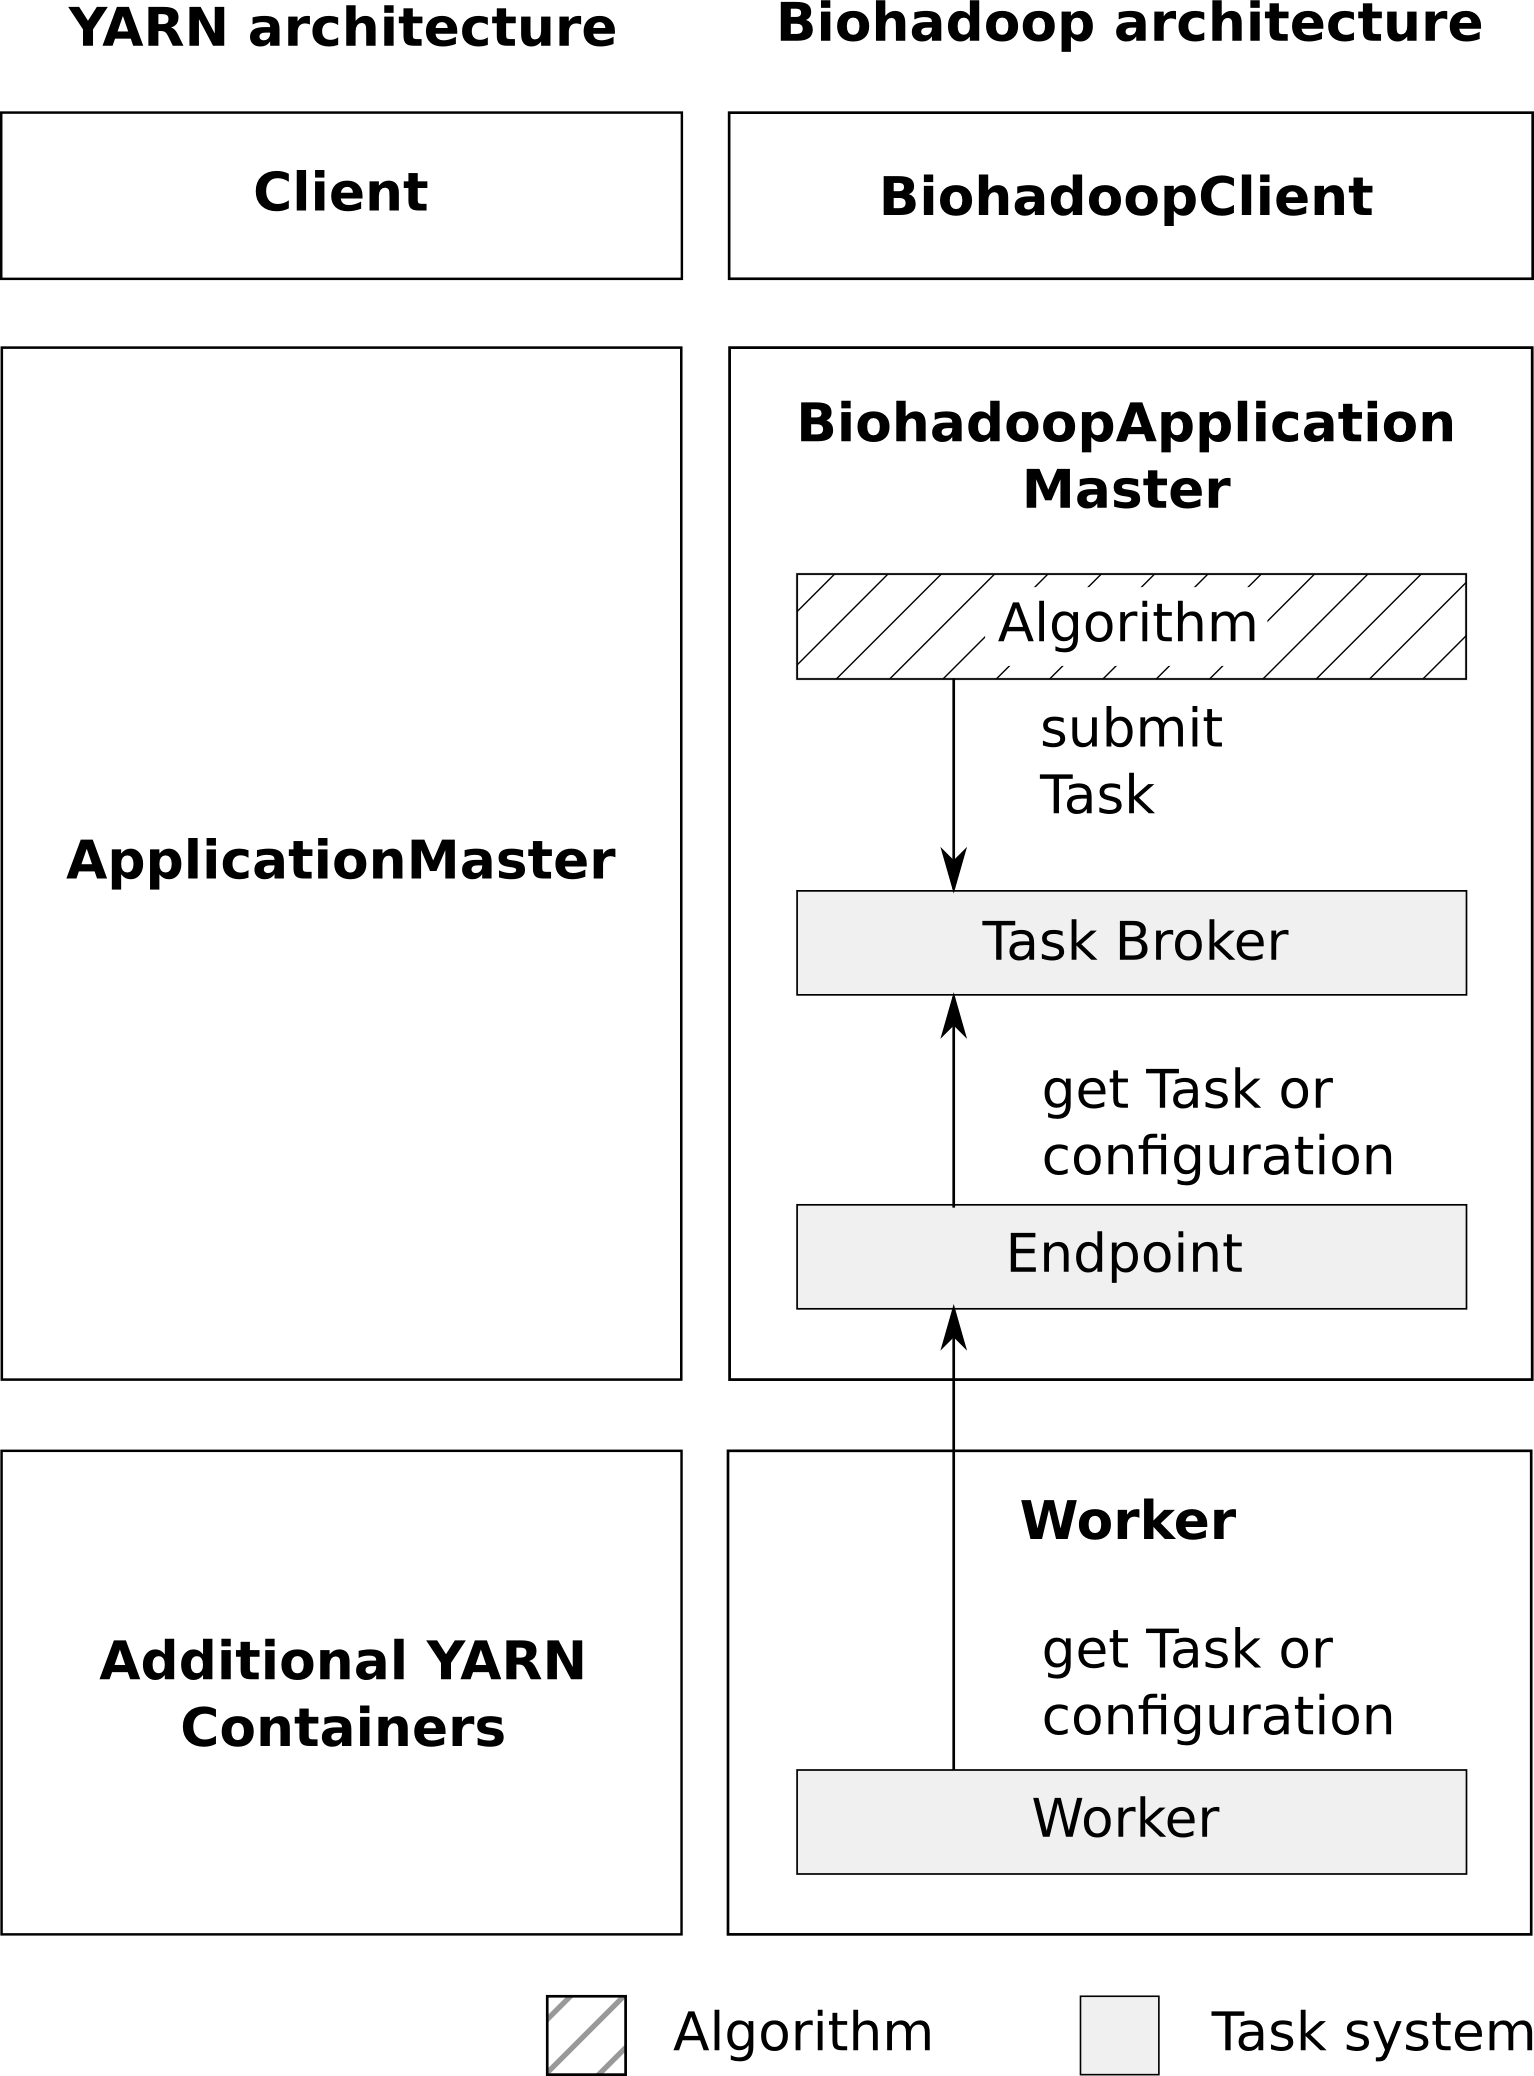
\includegraphics[width=90mm]{architecture.png}
    \caption{Biohadoop system architecture}
    \label{fig:architecture}
  \end{figure}
  
%   The whole task system runs in an asynchronous fashion, submitted tasks are not blocking the algorithm. Section \ref{chap:impl:task-system} describes the task system in detail
  
%   The tasks are actively requested by the workers, that communicate to their corresponding adapters. The adapters get the tasks out of the queues and deliver them to the workers. After the results are computed by the workers, those results are propagated back to the algorithm and the workers are free to request new tasks. The whole task system runs in an asynchronous fashion, submitted tasks are not blocking the algorithm. Section \ref{chap:impl:task-system} describes the task system in detail.\\

  
  \begin{figure}[ht!]
    \centering
    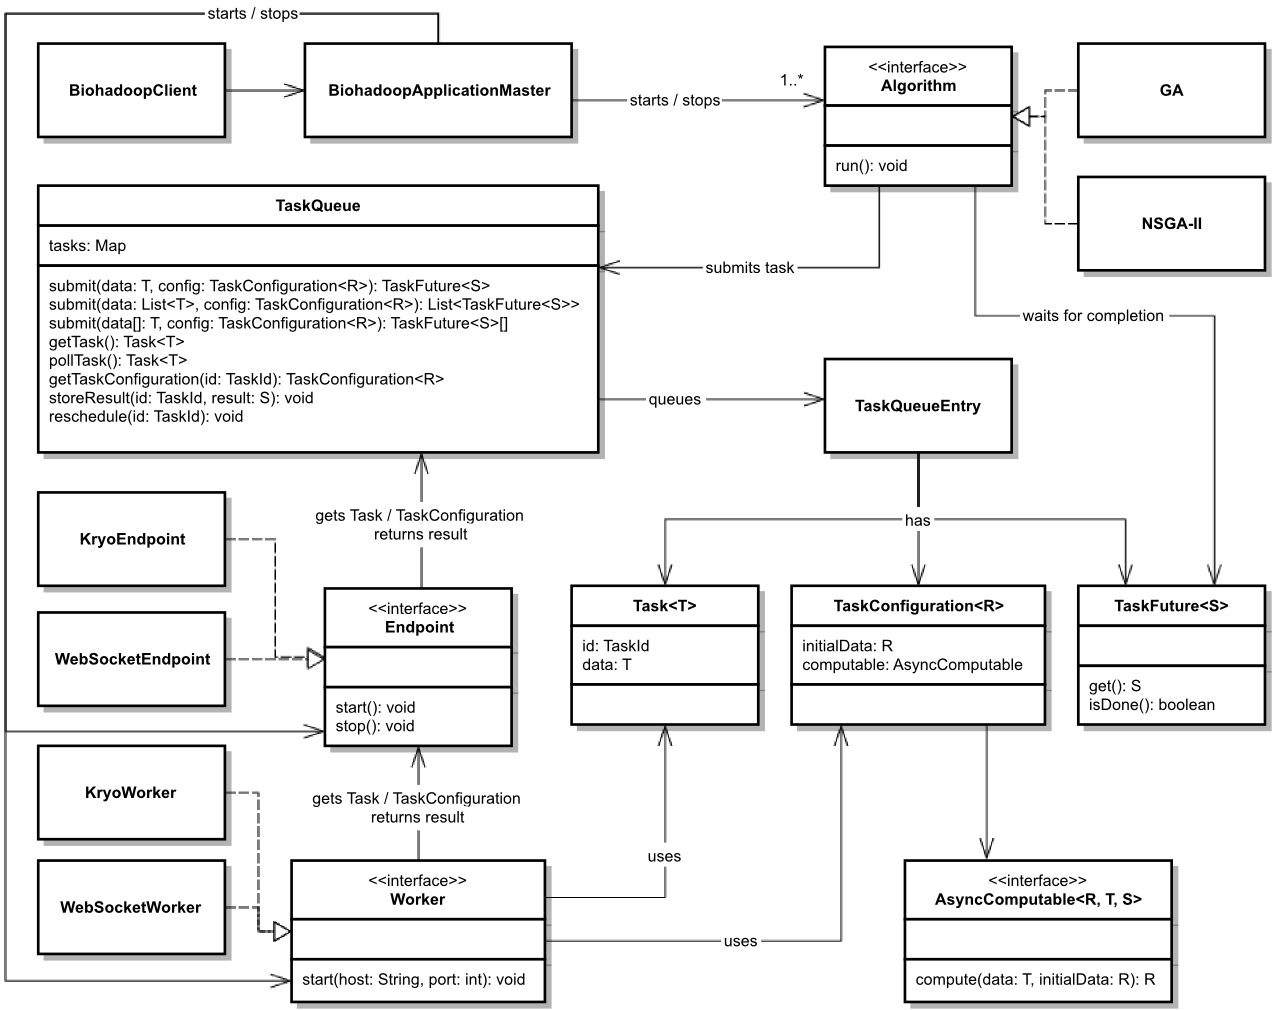
\includegraphics[width=140mm]{uml.png}
    \caption{Biohadoop UML Diagram}
    \label{fig:uml}
  \end{figure}
  
%   In addition, Figure \ref{fig:architecture} shows the architecture for offloading data from the main algorithm to local or remote workers. This is done by submitting chunks of data and a description of how to compute the results for this data chunks from the algorithm to the task system. In this architecture, the algorithm (section \ref{chap:impl:algorithm}) defines the problem that should be solved, e.g. an optimization problem. The data chunks, from here on called tasks, are smaller parts of this problem (e.g. compute the square root for a number), that can be submitted in an asynchronous fashion to the task system.
  
%   The task system consists of several parallel pipelines, whereas each pipeline is composed of task submitters, a task queue, adapters and workers. The tasks are actively requested by the workers, that communicate to their corresponding adapters. The adapters get the tasks out of the queues and deliver them to the workers. After the results are computed by the workers, those results are propagated back to the algorithm and the workers are free to request new tasks. The whole task system runs in an asynchronous fashion, submitted tasks are not blocking the algorithm. Section \ref{chap:impl:task-system} describes the task system in detail.\\
  
%   The task system relies on different communication mechanisms, to distribute the work among the waiting workers. Those communication mechanisms can be of any kind, whereas Biohadoop supports some types out of the box (local, HTTP, Kryo, Socket, Web Socket, as seen in figure \ref{fig:architecture}). The reason behind the decision to enable different kinds of communication mechanisms was, that all of them have different properties, and that for some workloads one may fit better then another. It is for example possible to distribute work to so called local workers. They are just threads and run inside the same JVM (Java Virtual Machine) as the algorithms, thus providing very little overhead to a solution that is implemented straight into the algorithm. By exposing a simple interface to the task system, changing later the type of worker (and with it the communication mechanism) to e.g. a remote type is just a matter of configuration. Another example would be when, during development, the socket communication is chosen. This is a performant way of communication, but may lead to firewall problems on some systems, as the right ports must be open. Changing this to use e.g. Web Sockets later on is, again, just a matter of configuration. More information about the communication mechanisms can be found in section \ref{chap:impl:communication}.\\


%  



% When an algorithm runs for a long time, it can be very annoying to lose results just because there was some kind of failure at any stage of computation. One solution to mitigate such problems is to save the current state of work to disk. Biohadoop supports its users in the task of saving and loading data with a set of classes and methods. One usage example is to reload the last state of an algorithm at startup, to continue the work at this point. To get more information about the persistence, refer to section \ref{chap:impl:persistence}.\\
%   
%   Biohadoop is capable of running several algorithms at the same time. They all run in the same JVM as Biohadoop does, and may be of the same type. As Hadoop on its own doesn't guarantee when a program runs, the mentioned capability of launching several algorithms at the same time in the same JVM is a useful enhancement when it comes to high level parallelization using the island model. If the algorithms were started by Hadoop one by one, it could be possible, that they were run in sequential order, instead of running at the same time.
%   
%   But Biohadoop doesn't restrict the usage of the island model to algorithms that run in the same JVM. By taking advantage of ZooKeeper \cite{zookeeper}, running algorithms may find each other also across the boundaries of different Biohadoop instances (Biohadoop can be started several times). This can lead to higher scalability, but entails the aforementioned problem, that Hadoop doesn't guarantee when a program runs, so a trade off has to be made. More information about how to use the island model in Biohadoop can be found in section \ref{chap:impl:island-model}\\
%   
%   To improve the understanding of the following sections, a simple example algorithm is introduced, called \texttt{Sum}. The algorithm takes an array of integers as input and provides the sum of them as result. For the sake of simplicity, we suppose that the input value of the \texttt{Sum} algorithm is never null. A simple implementation in Java can be found in listing \ref{listing:sum}, the output for different input values is given in table \ref{table:sum-algorithm}.
%   
%   \lstinputlisting[caption=Algorithm for integer summation,label=listing:sum]{../listings/chap4-sum.lst}
%   
%   \begin{table}
%     \centering
%     \setlength{\tabcolsep}{15pt}
%     \begin{tabular}{l|c}
%       numbers & sum \\ \hline
%       $[0]$ & $0$ \\
%       $[0,1]$ & $1$ \\
%       $[0,2,3]$ & $5$ \\
%     \end{tabular}
%     \caption{Example values for \texttt{Sum} algorithm}
%     \label{table:sum-algorithm}
%   \end{table}
% 
%   This example algorithm is good enough to demonstrate the usage of Biohadoop, other (more sophisticated) examples can be found at \cite{biohadoop-algorithms}. Chapter \ref{chap:usage} provides a step by step tutorial on how to implement this algorithm on Biohadoop.
%   
%   The following sections in this chapter continue to describe the implementation of Biohadoop in more detail, starting with the notion of Algorithm in section \ref{chap:impl:algorithm}. The next section \ref{chap:impl:task-system} talks about the task system, followed by the description of the communication mechanisms in section \ref{chap:impl:communication}. The enhancements section \ref{chap:impl:enhancements} talks about how Biohadoop supports persistence and the island model. How to configure Biohadoop is explained in section \ref{chap:impl:configuration}. If one just wants to use Biohadoop, chapter \ref{chap:usage} may be more helpful.
%   
% \section{Algorithm}
% \label{chap:impl:algorithm}
%   An algorithm in terms of Biohadoop is the implementation of an abstract problem that should be solved. For example, a genetic algorithm may be implemented to solve an optimization problem. Biohadoop supports the algorithm implementor with an easy way to parallelize the algorithm by providing an asynchronous task system (see \ref{chap:impl:task-system}). In addition, mechanisms for persistence and high level parallelization using an island model are offered (see \ref{chap:impl:enhancements}). All those capabilities can be used by the algorithm, but Biohadoop does not force their usage. The only thing an algorithm has to do to be run by Biohadoop, is to implement the \path{at.ac.uibk.dps.biohadoop.algorithm.Algorithm} interface, shown in listing \ref{listing:algorithm-interface}. This interface defines one method, which is invoked by Biohadoop after the system initialization has completed. There may run several algorithms of any kind at the same time in one Biohadoop instance, this is just a matter of configuration. After all algorithms have terminated, Biohadoop stops all components and shuts down.
% 
%   \lstinputlisting[caption=Algorithm interface,label=listing:algorithm-interface]{../listings/chap4-algorithm-interface.lst}
%   
%   \begin{itemize}
%     \item \texttt{void compute(SolverId solverId, Map<String, String>\newline configuration)}: This method is invoked by Biohadoop after the system initialization has completed. It is the place, where the algorithm should be implemented. The parameter \texttt{solverId} defines the global id of this instance of the algorithm, as there may run several instances of the same or different algorithms at the same time. The \texttt{solverId} can be used by other components to uniquely identify the algorithm. For example the persistence extension, which saves an algorithms state to a file, uses the \texttt{solverId} as part of the filename.
%     
%     The \texttt{properties} map contains the configuration for this algorithm (see \ref{chap:impl:configuration} for more information about how to configure Biohadoop). It is a map with key - value pairs of strings.
%     
%     The return value of the \texttt{compute} method is void, as there was no general return data identified, that could be useful. This may change in future versions.
%     
%     If there is an error during the algorithm execution, it may throw a  \path{at.ac.uibk.dps.biohadoop.algorithm.AlgorithmException} at any time. The meaning of a thrown \texttt{AlgorithmException} is, that there was an unrecoverable error which prevented the algorithm from progress, but the algorithm author was aware that such an error could happen, e.g. when a needed configuration argument is missing. Sometimes an algorithm may throw an unchecked exception, like the famous \texttt{NullPointerException}. The difference to \texttt{AlgorithmException} is in their semantics: unchecked exceptions are considered as the outcome of bugs. At the moment, Biohadoop makes no difference in handling \texttt{AlgorithmException} and unchecked exceptions, in both cases, the error is logged and the algorithm is terminated without affecting the other running algorithms. But it is possible that this behavior may change in the future. For example, it is thinkable that in the case of an \texttt{AlgorithmException}, a custom recovery procedure is invoked.
%   \end{itemize}
%   
%   When using the example algorithm from listing \ref{listing:sum}, without any further usage of the task system, persistence or high level parallelization, it would look like in listing \ref{listing:sum-biohadoop}. Note that there is no difference to the original implementation, except that now we have implemented the \texttt{compute(SolverId, Map<String, String>)} method.
%   
% 
%   \lstinputlisting[caption=\texttt{Sum} algorithm for integer summation on Biohadoop,label=listing:sum-biohadoop]{../listings/chap4-sum-biohadoop.lst}
% 
% \section{Task system}
% \label{chap:impl:task-system}
%   If an algorithm implementor decides to parallelize some parts of the algorithm, it can use Biohadoops task system. The task system works in an asynchronous manner and doesn't block its users while processing the tasks. However, it provides also mechanisms to block and wait for a result to be computed, if this is preferred.
%   
%   \subsection{Task pipeline}
%   \label{chap:impl:task-pipeline}
%   The task system is divided into several task pipelines, that run in parallel. Each pipeline has one or several task submitters, exactly one task queue, one or several adapters and one or several workers. Figure \ref{fig:single-pipeline} depicts the architecture of the task system with one task pipeline, consisting of one submitter, one queue, one adapter and one worker.
%   
%   \begin{figure}[ht!]
%     \centering
%     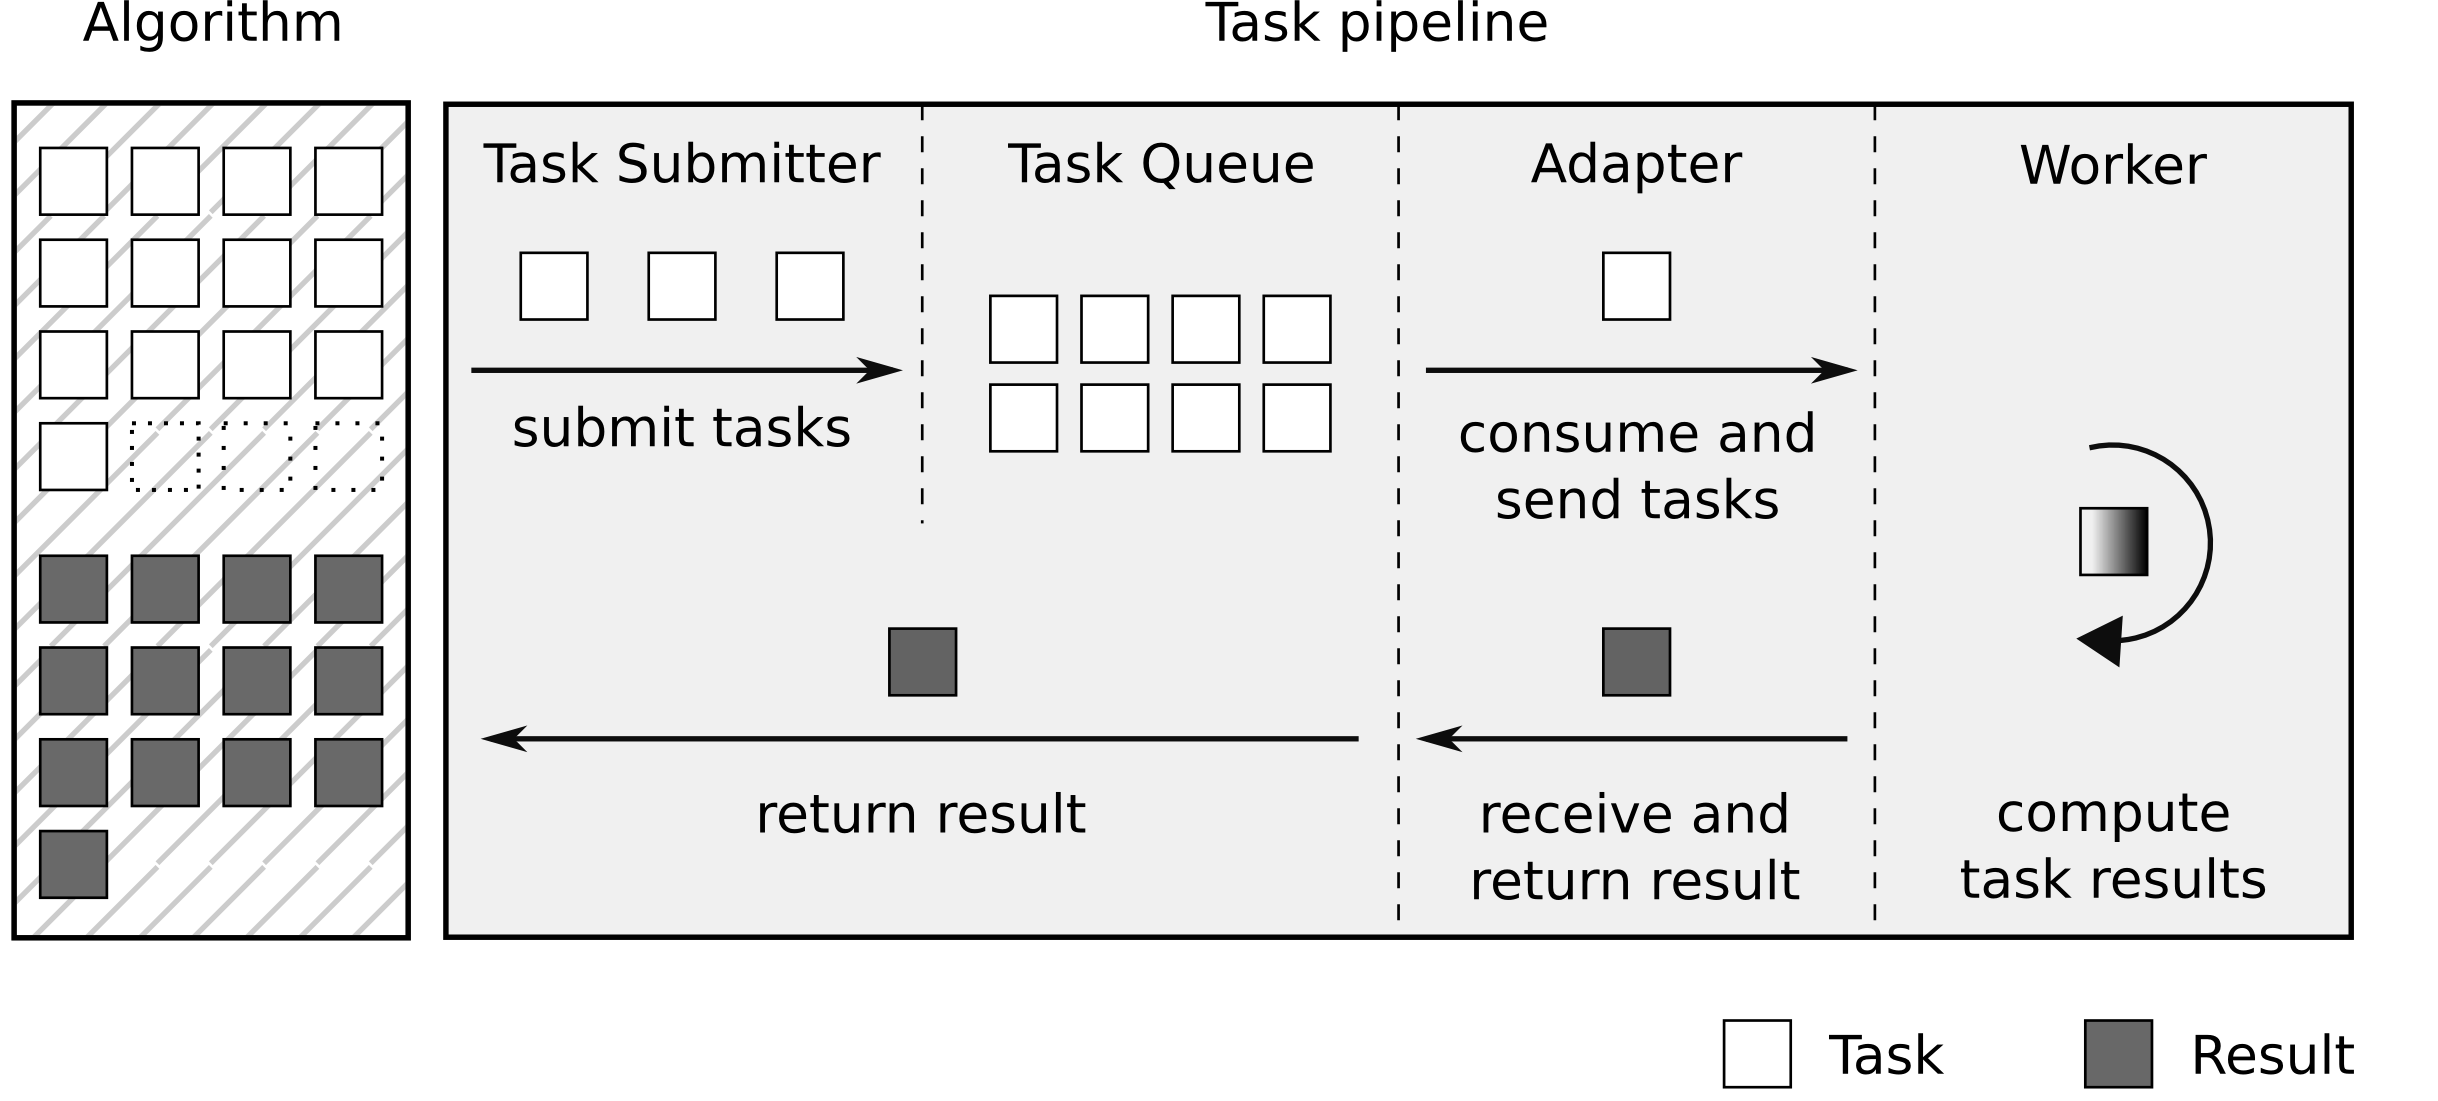
\includegraphics[width=130mm]{single-pipeline.png}
%     \caption{Task system with one task pipeline. The pipeline in this figure consists of one task submitter, one task queue, one adapter and one worker}
%     \label{fig:single-pipeline}
%   \end{figure}
%   
%   Central to each pipeline is the task queue. The queue is filled with tasks by the task submitters, that in turn get the tasks from the algorithm. Task submitters are a convenience abstraction that hide the complexity of task submission from the algorithm. An algorithm may choose to directly use a queue, although it is not recommended. Several submitters for one pipeline are supported.
%   
%   On the other side of the queue, we have the adapters and workers. The duty of the adapters is, to take tasks out of the queue and to pass them to the waiting workers, which do the (possibly heavy) computation of the tasks, and deliver the results back to the adapters. The adapters then propagate those results back to the algorithm. There may run several adapters and workers in each pipeline to enable parallel computation of the tasks. Each adapter can handle several workers.
%   
%   From the several parallel task pipelines, an algorithm can deliberately choose which one to use, it may use more then one. Figure \ref{fig:pipelines} for example depicts an algorithm, that uses four different task pipelines to handle its tasks, each pipeline consists of the before mentioned components. To enable the usage of several task pipelines in parallel and to distinguish them, unique names are used.
%   
%   \begin{figure}[ht!]
%     \centering
%     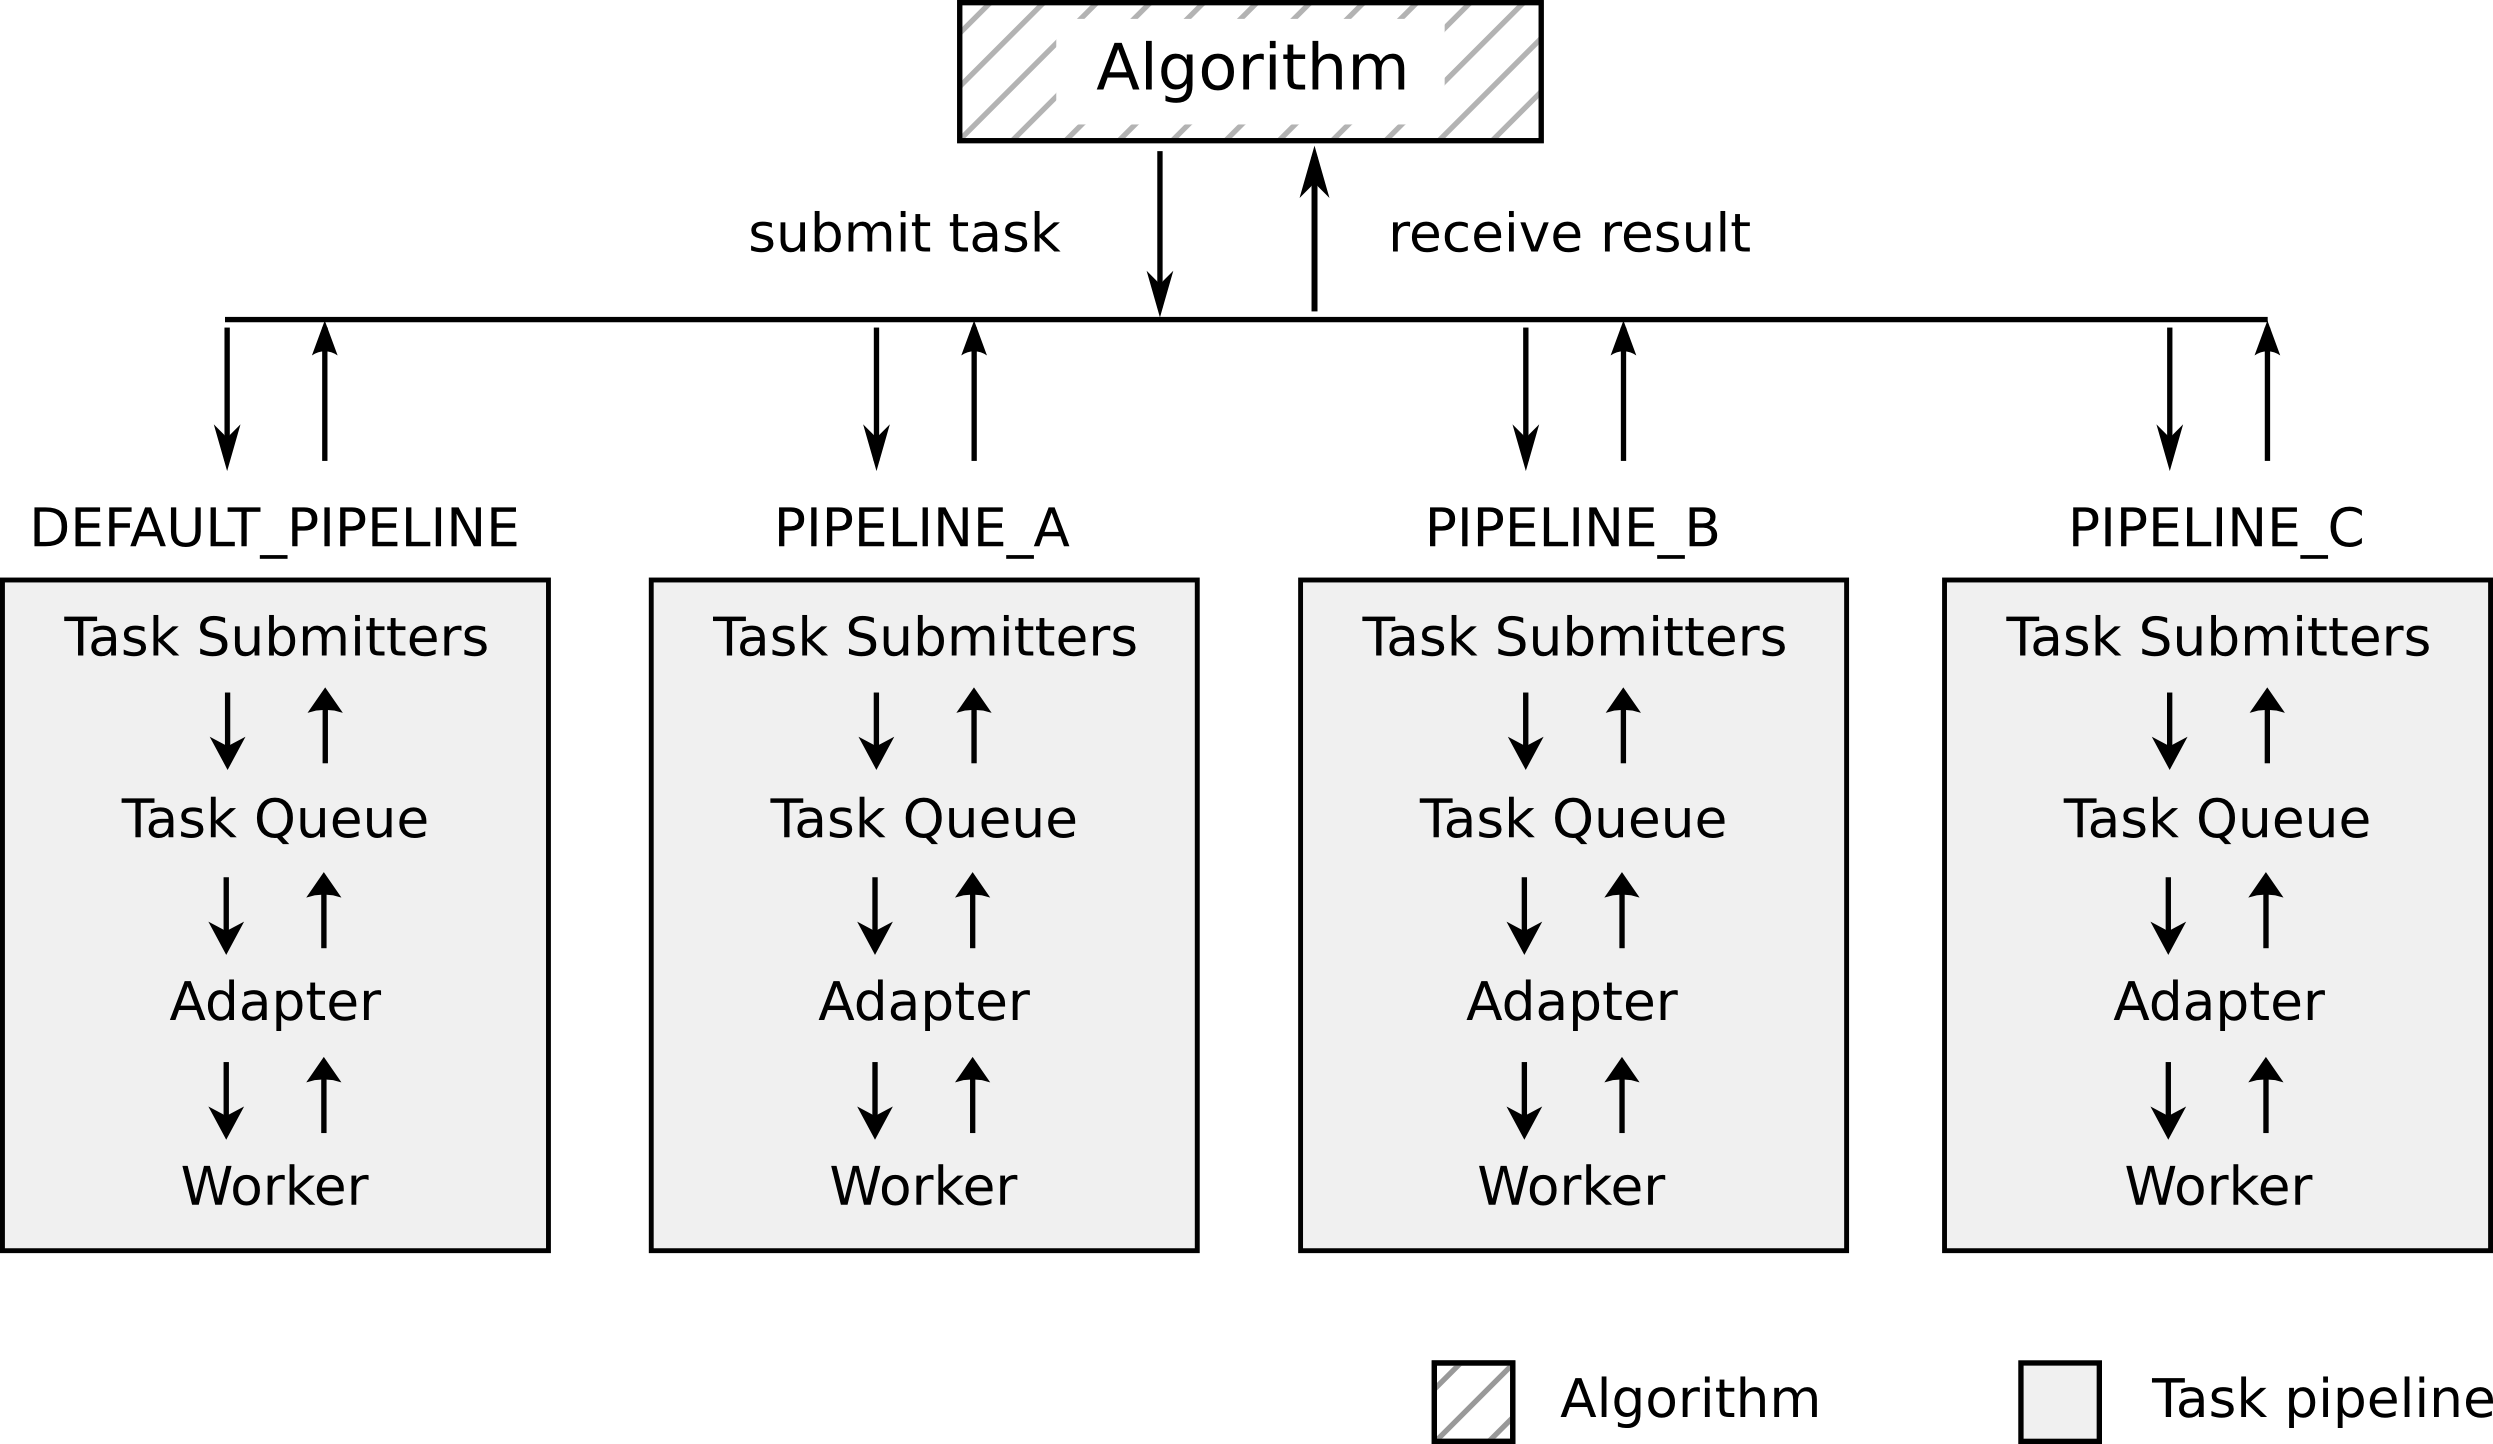
\includegraphics[width=130mm]{pipelines.png}
%     \caption{Several different named task pipelines may exist at the same time, consisting of submitters, queues, adapters and workers}
%     \label{fig:pipelines}
%   \end{figure}
% 
%   Every pipeline needs to be configured. To simplify this step, Biohadoop provides a pre-configured default pipeline, the \texttt{DEFAULT\_PIPELINE}. Using this default pipeline is advised, although it is possible to choose different pipelines for the task computation. Those other pipelines are from now on summarized under the term ``dedicated pipelines''. For example, the pipelines \texttt{PIPELINE\_A}, \texttt{PIPELINE\_B} and \texttt{PIPELINE\_C} in figure \ref{fig:pipelines} are dedicated pipelines, whereas the pipeline \texttt{DEFAULT\_PIPELINE} is the pre-configured default pipeline. All tasks submitted to the same pipeline share the same queue, adapters and workers.
%   
%   The main advantage of several parallel pipelines is better scalability. If one pipeline gets congested, a second pipeline, which works completely in parallel to the first one, can help to diminish this problem - given there are enough computational resources to effectively run the second pipeline. Another usage scenario for additional pipelines is, when there are tasks with different priorities, and one pipeline should only contain high priority tasks. By filling this pipeline only with high priority tasks, the tasks don't have to wait for other low priority tasks.
%   
%   The disadvantage of several pipelines is, that the workers of each pipeline receive only tasks from their pipeline. If no tasks are available (e.g. because there is not much work to do), then the workers have to wait, which can result in poor resource usage. Work stealing \cite{blumofe1999scheduling} between pipelines could reduce this problem, but is not implemented at the moment.
% 
%   Another disadvantage of dedicated pipelines is the slightly higher configuration effort, which really boils down to configure additional adapters and workers (more about this topic can be found in chapter \ref{chap:impl:configuration}, where the Biohadoop configuration is explained).
%   
%   In most cases, there is no need to run several pipelines and it is advised to start with the default pipeline. If there are good reasons, adding additional pipelines and dividing the tasks between them is straightforward.
%   
%   \subsection{Task Submitter}
%   \label{chap:impl:task-submitter}
%   The task submitter serves as the entry point to the task system and hides the complexity of the underlying components from the algorithm implementor. The generic interface \path{at.ac.uibk.dps.biohadoop.tasksystem.submitter.TaskSubmitter<T, S>}, shown in listing \ref{listing:taskSubmitter-interface}, defines the methods that a task submitter has to implement. T denotes the type of the task data, S denotes the type of the return value.
% 
%   \lstinputlisting[caption=TaskSubmitter interface,label=listing:taskSubmitter-interface]{../listings/chap4-taskSubmitter-interface.lst}
% 
%   \begin{itemize}
%     \item \texttt{TaskFuture<S> TaskSubmitter.add(T)}: This method adds a single task to a queue and returns a \texttt{TaskFuture}.
%     \item \texttt{List<TaskFuture<S>> TaskSubmitter.addAll(List<T>)}: This method adds a list of tasks to a queue and returns a list of \texttt{TaskFuture} objects, each one representing the result of exactly one submitted task. The tasks are then send one by one to the waiting workers.
%     \item \texttt{List<TaskFuture<S>> TaskSubmitter.addAll(T[])}: This method adds an array of tasks to a queue and returns a list of \texttt{TaskFuture} objects, each one representing the result of exactly one submitted task. The tasks are then send one by one to the waiting workers.
%   \end{itemize}
%   
%   \noindent
%   The methods of the \texttt{TaskSubmitter} interface return objects that implement \path{at.ac.uibk.dps.biohadoop.tasksystem.queue.TaskFuture<T>}, shown in listing \ref{listing:taskFuture-interface}, where T is the type of the return value. A \texttt{TaskFuture} object represents the result of an asynchronous computation performed by a worker, much like the \path{java.util.concurrent.Future} object, that is part of the Java standard.
% 
%   \lstinputlisting[caption=TaskFuture interface,label=listing:taskFuture-interface]{../listings/chap4-taskFuture-interface.lst}
% 
%   \begin{itemize}
%     \item \texttt{T get()}: Is used to wait until the result of a remote computation is available, which leads to a blocking behavior. After the result is available, \texttt{get()} returns this result.
%     \item \texttt{boolean isDone()}: Is used to check the task status, by which a non-blocking behavior can be realized. When \texttt{isDone()} returns true, the result can be obtained by invoking \texttt{get()} on the \texttt{TaskFuture} object.
%   \end{itemize}
% 
%   \noindent
%   The following code snippet illustrates a simple example, where a task is submitted to a queue, after which the program blocks until the result arrives by invoking \texttt{get()}. We assume here, that \texttt{taskSubmitter} is an initialized object that implements the \texttt{TaskSubmitter} interface. Further we assume, that the task data type is \texttt{String} and the return type is \texttt{int}:
%   \begin{lstlisting}
%     int result = taskSubmitter.add("Hello World!").get();
%   \end{lstlisting}
% 
%   The default implementation of the \texttt{TaskSubmitter} interface, that is provided by Biohadoop, is  \path{at.ac.uibk.dps.biohadoop.tasksystem.queue.SimpleTaskSubmitter}. It provides three different constructors that can be used to configure the details of task submission e.g. to which task pipeline a task is submitted. See listing \ref{listing:simpleTaskSubmitter} for more details about the constructors.
%   
%   \lstinputlisting[caption=SimpleTaskSubmitter,label=listing:simpleTaskSubmitter]{../listings/chap4-simpleTaskSubmitter.lst}
%   
%   As one can see, all constructors expect as parameter at least a class that extends the \path{at.ac.uibk.dps.biohadoop.tasksystem.AsyncComputable} interface. This class implements the part of the algorithm, that should be run on the workers and that is used to compute the results for the submitted tasks (more information about this interface and its usage can be found at section \ref{chap:impl:async-computable}).
%   
%   The second constructor expects an object containing the initial data, \texttt{initialData}, that should be available in the \texttt{AsyncComputable} class and therefore on the workers. This is suitable when several tasks need the same data for their computation, that doesn't change over time. The \texttt{initialData} is send to the workers when they first encounter a task that should be computed with a given \texttt{AsyncComputable} class. After that, this \texttt{initialData} is cached at the workers.
%   
%   For an example usage of the \texttt{initialData}, lets suppose we write an algorithm, that computes, for a list of locations, the distances to the nearest city and returns the nearest city. As input we have a list of cities with their coordinates (called \texttt{CITY\_LIST}), and a list of locations with their coordinates (called \texttt{LOCATION\_LIST}). This problem can be parallelized by breaking the list of locations down to single locations, for which the results can be computed in parallel. To get the nearest city for a given location, the algorithm computes the distances to all cities, and returns the city with the smallest distance. This algorithm could be implemented and parallelized with Biohadoop and its task system, where the task of computing the smallest distance for a given location is done by workers. Now, the \texttt{CITY\_LIST} remains the same for all locations, so it would be a bad idea to send the \texttt{CITY\_LIST} data to the workers for every task. This is the reason why the \texttt{initialData} exists: we set \texttt{CITY\_LIST} as initial data for the task submission and it gets transferred to a worker the first time it encounters this type of task (namely to compute the distance). After this first time, the \texttt{CITY\_LIST} can be reused by the worker, without the need to transmit it over and over. This usually results in much less overhead when the next task of this type has to be computed by the worker.
%   
%   The last constructor expects an additional \texttt{pipelineName} argument, that defines to which task pipeline the tasks, submitted using this task submitter, should be send. Using this constructor, an algorithm implementor is able to choose a dedicated pipeline for the task computation. Constructors that take no \texttt{pipelineName} argument, submit their tasks to the default pipeline.
%   
%   \subsection{Task Queue}
%   Tasks, submitted by the algorithms to be processed by the task system, are stored in task queues. The queue, where a task is stored, is part of the same pipeline as the task submitter, that put the task into the queue. There may exist several task queues, each queue is assigned to one task pipeline, which uses the queue exclusively during their whole lifetime. All tasks submitted to a given task queue have the same priority. Stored tasks are consumed by adapters and, from there on, handed to the workers for computation.
%   
%   Each task queue works as a first-in first-out (FIFO) queue. The head of the queue is that element, that has been on the queue the longest time. The tail of the queue is that element, that has been on the queue the shortest time. New elements are inserted at the tail of the queue. When reading from the queue, the head element is taken out of the queue and returned as result.
%   
%   Every task queue is backed by \path{java.util.concurrent.LinkedBlockingQueue}, which supports at maximum $2^{31} - 1$ number of elements, in this case tasks. The \texttt{LinkedBlockingQueue} supports concurrent addition and retrieval of elements. This facilitates the usage of many task submitters and adapters per queue. The \texttt{LinkedBlockingQueue} may block when adding an element and the queue is already full, or when an element should be taken out of an empty queue. In this two corner cases, also the task queue blocks. This may lead to the following problems:
%   \begin{itemize}
%     \item The task queue blocks when an algorithm wants to submit new tasks to a full queue. This kind of problem may arise if there is a huge number (more than $2^{31} - 1$) of tasks that are added to a task pipeline way faster than they can by computed. As a result, the algorithm gets also blocked and has to wait for free space in the task queue. This is a seldom case, but if it happens, there is the possibility to distribute the work between several task pipelines (and therefor between several queues), or to do the task submission in an own thread (could be implemented e.g. in a \texttt{TaskSubmitter}).
%     \item The task queue blocks, when an adapter wants to take a task out to send it to a waiting worker, but the queue is empty. This case happens often and results in blocking behavior of the adapters and workers. Adapters should therefor be prepared for this case and nevertheless at least accept new worker requests (Biohadoops provided adapters work in this manner). A way to diminish the blocking behavior would be to implement some kind of work stealing between queues, that is, an empty queue may fetch tasks from other queues that contain elements. This is not implemented at the moment. As a result, workers block if there is no work to do for their pipeline.
%   \end{itemize}
%   
%   As mentioned in the chapter before, it is preferable to submit tasks to a task queue by using the provided \path{at.ac.uibk.dps.biohadoop.tasksystem.queue.SimpleTaskSubmitter}, although it is not necessary. It is still possible to submit tasks directly to a task queue. To do this, first a reference to a task queue must be retrieved. This can be done by using the \texttt{at.ac.uibk.dps.biohadoop.tasksystem.queue.TaskQueueService}, which is a singleton and provides methods as seen in listing \ref{listing:taskQueueService}. Please keep in mind that the rest of this section is for advanced users only and may be skipped.
%   
%   \lstinputlisting[caption=TaskQueueService,label=listing:taskQueueService]{../listings/chap4-taskQueueService.lst}
%   
%   \begin{itemize}
%     \item \texttt{getInstance()}: is used to get an instance of the \texttt{TaskQueueService} singleton.
%     \item \texttt{TaskQueue<R, T, S> getTaskQueue(String name)}: this method provides a reference to a task queue with the given name. If no such task queue exists, a new one is created.
%     \item \texttt{stopAllTaskQueues()}: this method stops all task queues and should not be invoked by an algorithm implementor. It is used internally by Biohadoop in the shutdown process. When this method is called, all workers get notified to shut down. In addition, the task queue is removed from the internal storage and if there are no other references to this queue, it is made available for garbage collection.
%   \end{itemize}
% 
%   By invoking \texttt{getTaskQueue(String)} on the \texttt{TaskQueueService} singleton, a reference to a generic task queue is retrieved, which is of type \path{at.ac.uibk.dps.biohadoop.tasksystem.queue.TaskQueue}. The task queue offers the methods in listing \ref{listing:taskQueue}. The \texttt{add...()} methods are useful to submit new tasks, the  \texttt{stopQueue()} can be used to stop the queue and all of its depending workers. The other methods are usually used by adapters. When invoking the  \texttt{add...()} methods, new objects of type \path{at.ac.uibk.dps.biohadoop.tasksystem.queue.ClassNameWrappedTask} are created, that wrap the actual data, the information about which class to use to compute the result and a unique id. Those task objects can be retrieved by using the \texttt{getTask()} method.
%   
%   The generic types of the \texttt{TaskQueue} are T, which denotes the type of the task data, S denotes the type of the return value and R denotes the type of the inital data.
%   
%   \lstinputlisting[caption=TaskQueue,label=listing:taskQueue]{../listings/chap4-taskQueue.lst}
%   
%   \begin{itemize}
%     \item \texttt{add(T data, String asyncComputableClassName, R initialData) throws InterruptedException}: adds \texttt{data} of type T to the task queue, where \texttt{asyncComputableClassName} is the name of the class that should be used by the workers to compute this task. \texttt{initialData} is the data that is send to a worker when it first encounters this \texttt{asyncComputableClassName}. The method returns a \texttt{TaskFuture} object that represents the result of the computation (see chapter \ref{chap:impl:task-submitter} for more information about the \texttt{TaskFuture}). This method may throw an \texttt{InterruptedException}, if the underlying queue is interrupted while the task is inserted.
%     \item \texttt{addAll(List<T> datas, String asyncComputableClassName,\newline R initialData) throws InterruptedException}: adds a list of \texttt{datas} of type T to the task queue, where \texttt{asyncComputableClassName} is the name of the class that should be used by the workers to compute this tasks. \texttt{initialData} is the data that is send to a worker when it first encounters this \texttt{asyncComputableClassName}. The method returns a list of \texttt{TaskFuture} objects, each one representing the result of a computation. This method may throw an \texttt{InterruptedException}, if the underlying queue is interrupted while the task is inserted.
%     \item \texttt{addAll(T[] datas, String asyncComputableClassName,\newline R initialData) throws InterruptedException}:  adds an array of \texttt{datas} of type T to the task queue, where \texttt{asyncComputableClassName} is the name of the class that should be used by the workers to compute this tasks. \texttt{initialData} is the data that is send to a worker when it first encounters this \texttt{asyncComputableClassName}. The method returns a list of \texttt{TaskFuture} objects, each one representing the result of a computation. This method may throw an \texttt{InterruptedException}, if the underlying queue is interrupted while the task is inserted.
%     \item \texttt{getTask() throws InterruptedException}: gets the next \texttt{Task} object out of the task queue and returns it as result. This method may throw an \texttt{InterruptedException}, if the underlying queue is interrupted while the task is retrieved.
%     \item \texttt{getInitialData(TaskId taskId) throws TaskException}: this method gets the initial data for a task with the given \texttt{TaskId}. The \texttt{TaskId} is an internal id that is unique for every task. \texttt{Task} objects, that are returned by the \texttt{getTask()} method, encapsulate this \texttt{TaskId}.
%     \item \texttt{storeResult(TaskId taskId, S data)}: is used to store the result of the computation for the task with the given \texttt{TaskId}.
%     \item \texttt{reschedule(TaskId taskId) throws InterruptedException,\newline TaskException}: if something goes wrong while computing the result for a task, this task can be rescheduled, so it can be computed again. This method is useful e.g. in error conditions. It may throw an \texttt{InterruptedException}, if the underlying queue is interrupted while the task is inserted. It may throw a \texttt{TaskException} if the given \texttt{TaskId} is unknown to this task queue.
%     \item \texttt{stopQueue()}: stops this queue and notifies all workers to shut down.
%   \end{itemize}
% 
%   As one can see, the methods offered by the \texttt{TaskQueue} are rather low level. Direct usage of the \texttt{TaskQueue} is advised only if Biohadoop should be extended for example with new task submitters or new adapters.
%   
%   \subsection{Adapter}
%   \label{chap:impl:adapter}
%   An adapter takes tasks out of a queue and passes it to waiting workers through some kind of communication facility. The results returned by the workers are than handed back to the algorithm. So the most important aspect of an adapter is to communicate with the corresponding workers. This communication can be of any kind, and its technical details are hidden from an algorithm implementor. Already implemented examples for such communication types are HTTP, Kryo, Socket, WebSocket, but also simple variable sharing when the communication is done between different threads in the same JVM. Section \ref{chap:impl:communication} talks in greater detail about the communication aspects.
%   
%   As explained in the previous sections, there may be several task pipelines. Each pipeline consists of task submitters, a queue, the adapters and workers. Because of this rather tight coupling of queue, adapters and workers, adapters must be configured in a way, such that they know from which queue they should take the work. The default pipeline needs no configuration, for the configuration of a dedicated pipeline, take a look at section \ref{chap:impl:configuration}. There is no restriction on the number of running adapters.
%   
%   The communication types provided by Biohadoop should be enough for the average needs. But if one wants to use a different communication type, an implementation of the adapter and worker is needed. For the adapter side of the communication, this can be done through implementing the interface \path{at.ac.uibk.dps.biohadoop.tasksystem.adapter.Adapter}, shown in listing \ref{listing:adapter-interface}. Be aware that the methods in this interface are called by Biohadoop, so there is no need to call them somewhere manually, they are part of the life cycle of an adapter. This life cycle methods are called by Biohadoop in a sequential manner throughout all configured adapters, if one call blocks, the whole Biohadoop system blocks. The communication between adapter and workers is not part of this interface and can be designed as needed.
%   
%   Figure \ref{fig:flow-adapter} depicts the typical life cycle of an adapter. If any \texttt{configure(String)} or \texttt{start()} method throws an exception (in contrast to the figure), Biohadoop terminates at this point.
%   
%   \begin{figure}[ht!]
%     \centering
%     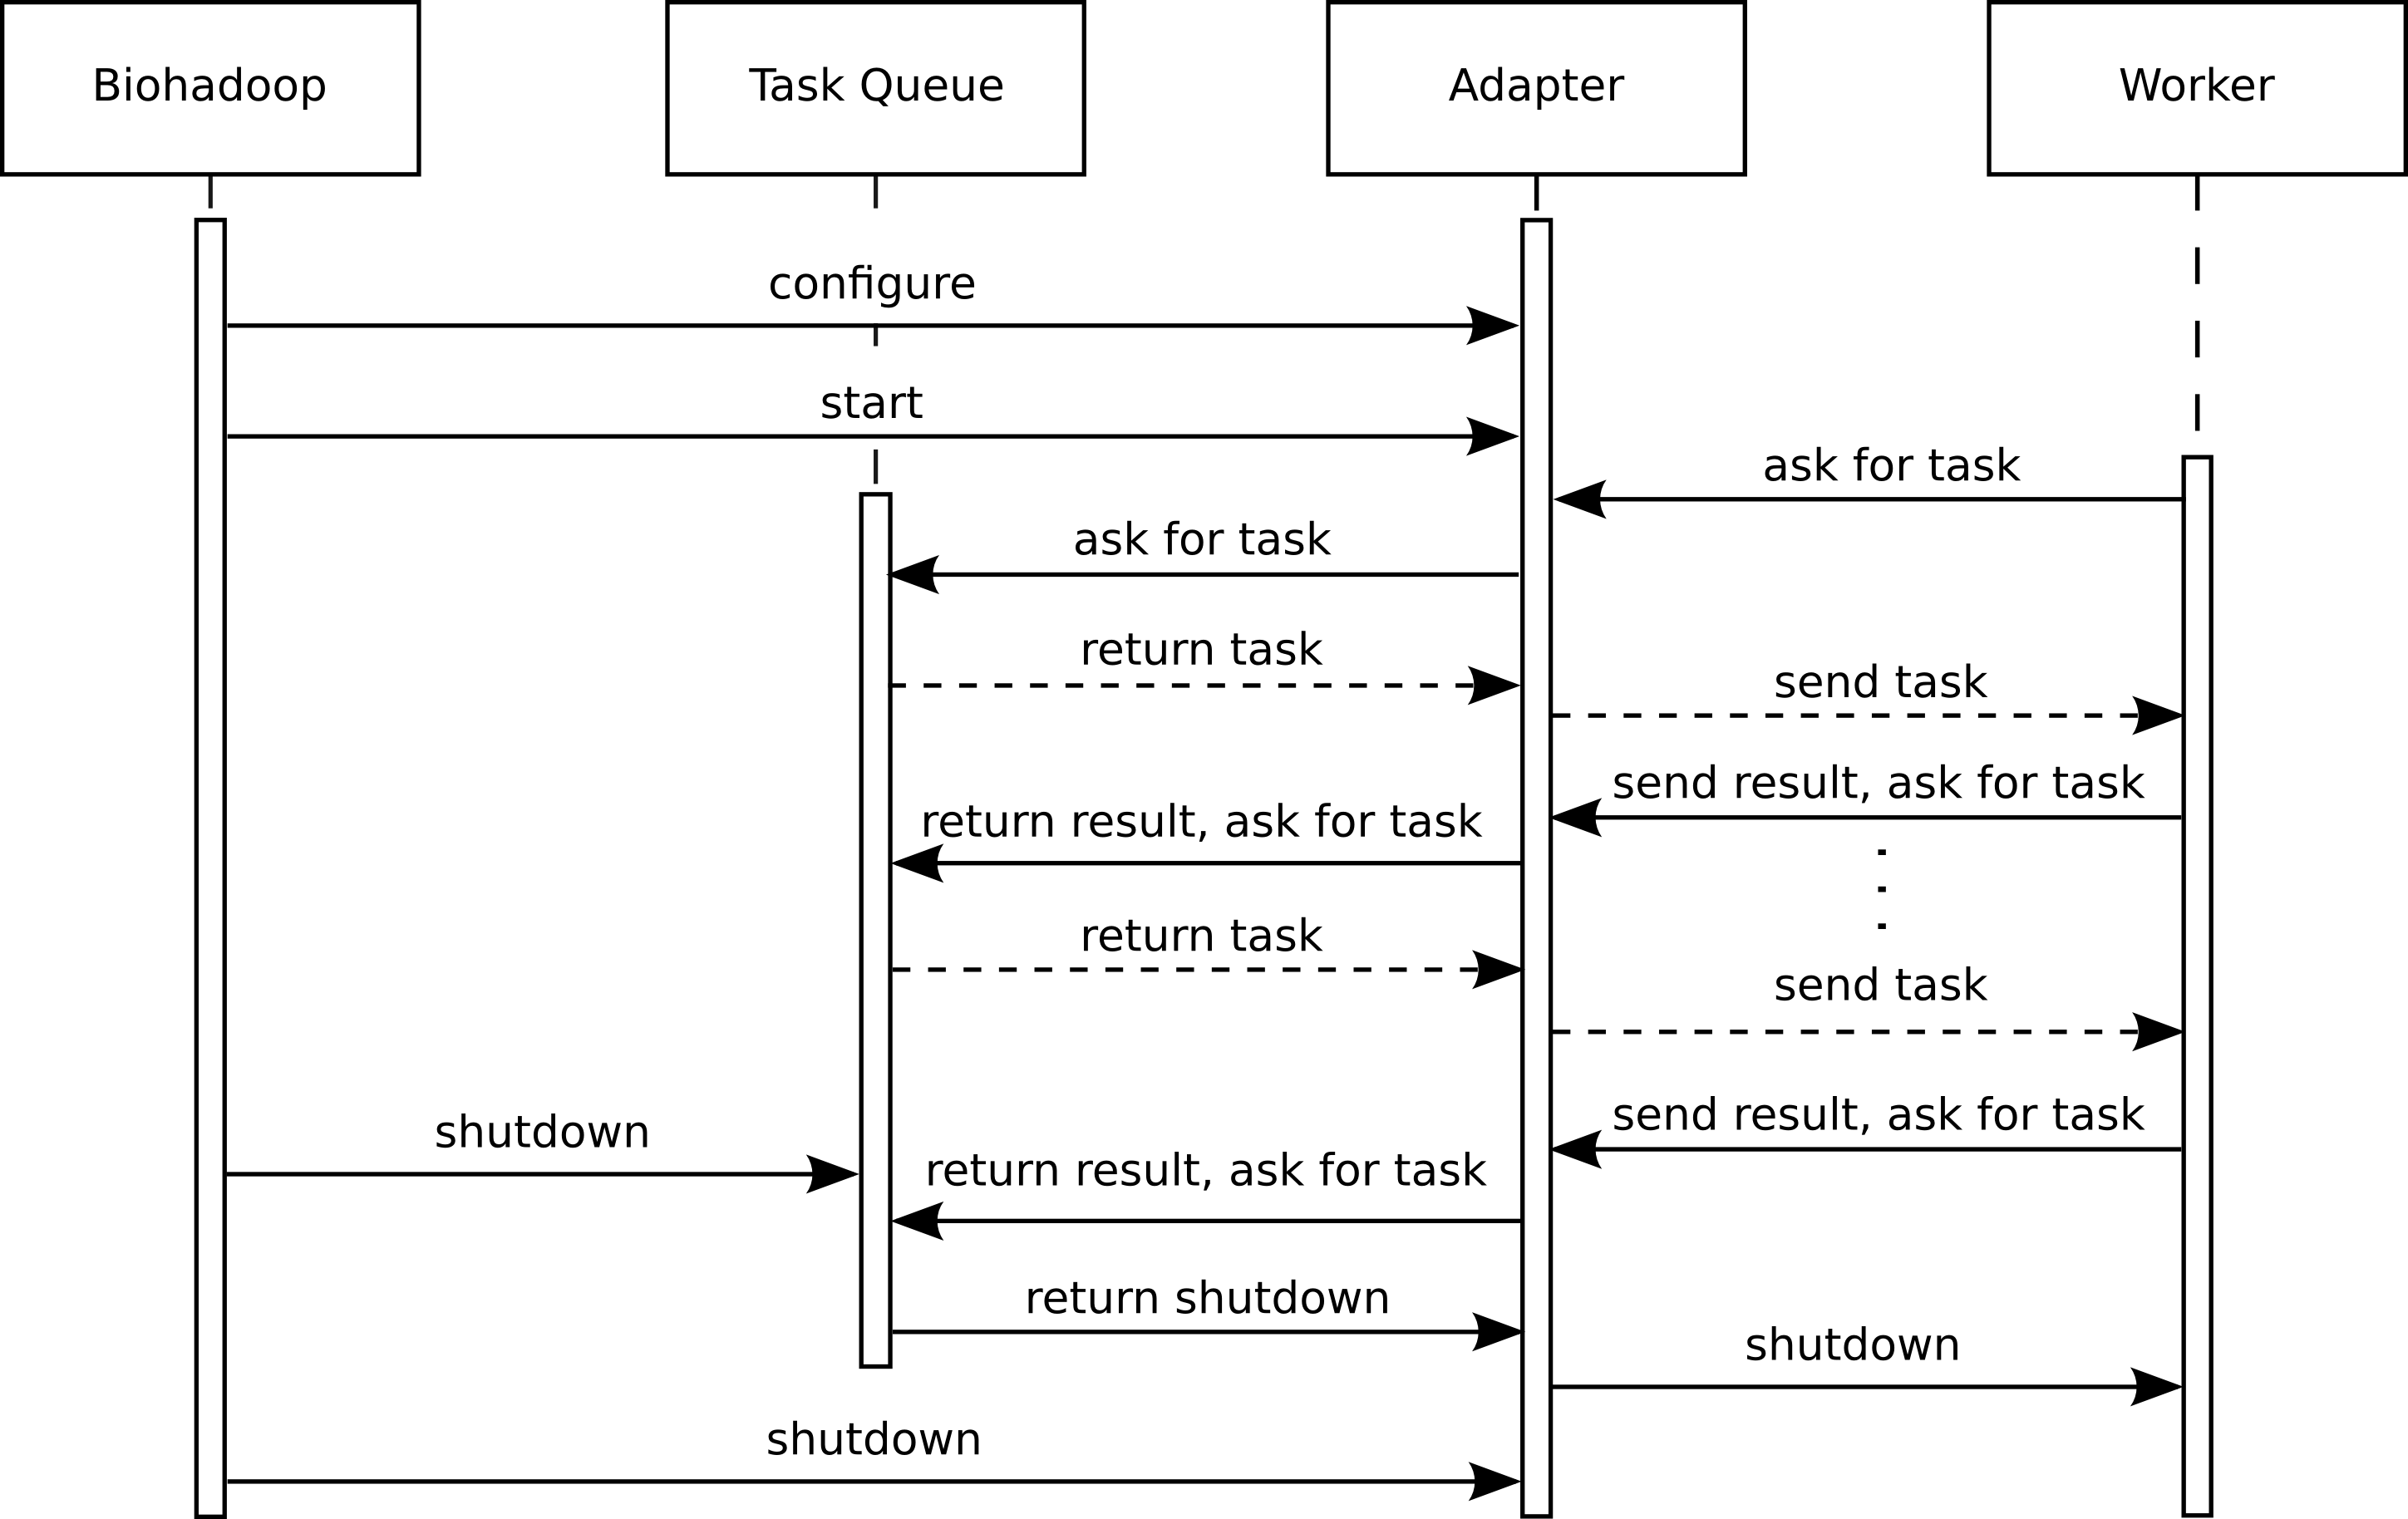
\includegraphics[width=130mm]{flow-adapter.png}
%     \caption{Life cycle of an adapter}
%     \label{fig:flow-adapter}
%   \end{figure}
%   
%   \lstinputlisting[caption=Adapter interface,label=listing:adapter-interface]{../listings/chap4-adapter-interface.lst}
% 
%   \begin{itemize}
%     \item \texttt{void configure(String pipelineName) throws AdapterException}: this method is called by Biohadoop when it prepares all the configured adapters. It provides a \texttt{pipelineName}, that defines the pipeline to which the adapter belongs. In addition, this is by convention the queue name, from which the adapter should consume the tasks. In this method, an adapter may initialize its behavior, but it should not start working (e.g. open a socket). It may throw a \texttt{AdapterException}, which leads Biohadoop to shutdown completely. Any other uncatched exception also leads to a complete shutdown. This is done to comply with the fail fast principle of application behavior \cite{shore2004fail}, which leads in this case to a system that is either running fully functional or not running at all.
%     \item \texttt{void start() throws AdapterException}: this method is called by Biohadoop to start all of the configured adapters. It is the right place to start up the adapters part of the communication, e.g. to open a listening socket. The method may throw a AdapterException which leads to a complete shutdown. Again, every uncatched exception also leads to a complete shutdown.
%     \item \texttt{void stop()}: This method is called by Biohadoop after all algorithms are finished, no matter if they threw an exception or not. In this method, the communication facility (e.g. socket) should be closed.
%   \end{itemize}
%   
%   \subsection{Worker}
%   \label{chap:impl:worker}
%   The workers implement the asynchronous (and possibly parallelized) part of the algorithm and actively request new tasks from the adapters. If the adapters have currently no work to offer, for example because the running algorithms have not submitted any tasks to the task system, then the workers wait until new work is available. Of course, the workers need some resources during the waiting times too (in terms of CPU, RAM, storage and so on), so when running Biohadoop, one should consider how much workers are really needed and at which point more of them are counterproductive.
%   
%   There are two different kinds of workers: the ones that run under the control of the Apache Hadoop system, (from now on called embedded workers) and the ones that run from outside of this system (from now on called external workers), Biohadoop supports both forms. Embedded workers must be configured in Biohadoop, but then the whole startup and shutdown is done automatically. In contrast, external workers don't have to be configured by Biohadoop, but their whole life cycle must be controlled in some other way, which is not part of Biohadoop. This can pose some problems, as external workers need to know e.g. when and where Biohadoop is running and how to connect to its running adapters. If there are no special needs, embedded workers are just fine. There are although some good reasons to use external workers:
%   
%   \begin{itemize}
%     \item external worker don't necessarily depend on the Hadoop ecosystem, they may run wherever they want, as long as they are able to communicate to at least one adapter. It is possible to develop external workers, that run in completely different environments for example mobile phones.
%     \item there is no restriction on the program language for an external worker, as long as it knows how to talk to at least one adapter. For example it is possible to implement a worker in JavaScript \cite{bioworker-browser} or Python \cite{bioworker-python}. In contrast to this, embedded workers have to be written in Java.
%     \item there is no limit in the number of external workers that may run. With suited algorithms to solve, this can lead to enormous scale. The algorithm should be suited in the sense, that the tasks are not to short running, as this would lead to high network traffic, effectively making this the bottleneck. The number of embedded workers is limited by the Hadoop environment, on which Biohadoop runs.
%   \end{itemize}
% 
%   Crucial to external workers is the fact, that they have to know how to communicate to the adapters. As it is not always easy to simulate e.g. the Java serialization mechanism in other languages, there are different kinds of adapters, that run different types of communication facilities. The most straight forward type of communication is using HTTP, a protocol for which there is an implementation in almost every language of the world. This way it is possible to implement external workers in a broad range of programming languages.\\
%   
%   
%   !!!!Workers don't get restarted if they fail!!!!\\
%   
%   
%   Embedded workers must implement the interface \path{at.ac.uibk.dps.biohadoop.tasksystem.worker.WorkerEndpoint}, that is shown in listing \ref{listing:worker-interface}.
% 
%   \lstinputlisting[caption=Worker interface,label=listing:worker-interface]{../listings/chap4-worker-interface.lst}
%   
%   \begin{itemize}
%     \item \texttt{String buildLaunchArguments(WorkerConfiguration\newline workerConfiguration) throws WorkerLaunchException}: this method is called by Biohadoop before the startup of the worker. The return value is a String, that contains needed configuration options for the worker to start. This string is provided to the worker at its startup. The reason for this method to exist is, that it is called inside the Biohadoop process, which opens the possibility to make use of Biohadoop internal configuration options and variables. After an embedded worker is started by Biohadoop (using the Hadoop YARN capabilities) it runs in a separated process on perhaps a different machine, and has no easy way to access the internal Biohadoop state. The method may throw a \texttt{WorkerLaunchException}, after which the whole Biohadoop system shuts down, in order to adhere to the fail fast principle. Every other uncatched exception also leads to the complete shutdown of Biohadoop.
%     \item \texttt{void configure(String[] args) throws WorkerException}: this method is called, after the embedded worker is instantiated i.e. when it is already running as a separate process on perhaps a different machine. The method takes an array of Strings as input parameters, which is exactly the array of Strings used to instantiate the worker process, or in other words, these are the parameters provided to the static \texttt{main(String args[])} method of the worker at startup. The arguments contain, beside the arguments of the \path{buildLaunchArguments(WorkerConfiguration)}, additional values, that may be useful, e.g. the path to Biohadoops config file. The method may throw a WorkerException, after which this worker is terminated and an error code of 1 is returned to Biohadoop.
%     \item \texttt{void start() throws WorkerException,\newline ConnectionRefusedException}: this method starts the main loop of the worker, where it begins to request tasks from the corresponding adapters. Usually, the adapter notifies the worker when to shutdown, which leads the worker to exit this method and to terminate its process with an exit code of 0. The method may throw a WorkerException after which this worker is terminated and an error code of 1 is returned to Biohadoop. It may throw a ConnectionRefusedException if it is unable to connect to its adapter. In this case, the worker shuts down, and an error code of 2 is returned to Biohadoop. Every other uncatched exception also shuts the worker down and returns an error code of 1 to Biohadoop.
%   \end{itemize}
%   
%   \begin{figure}[ht!]
%     \centering
%     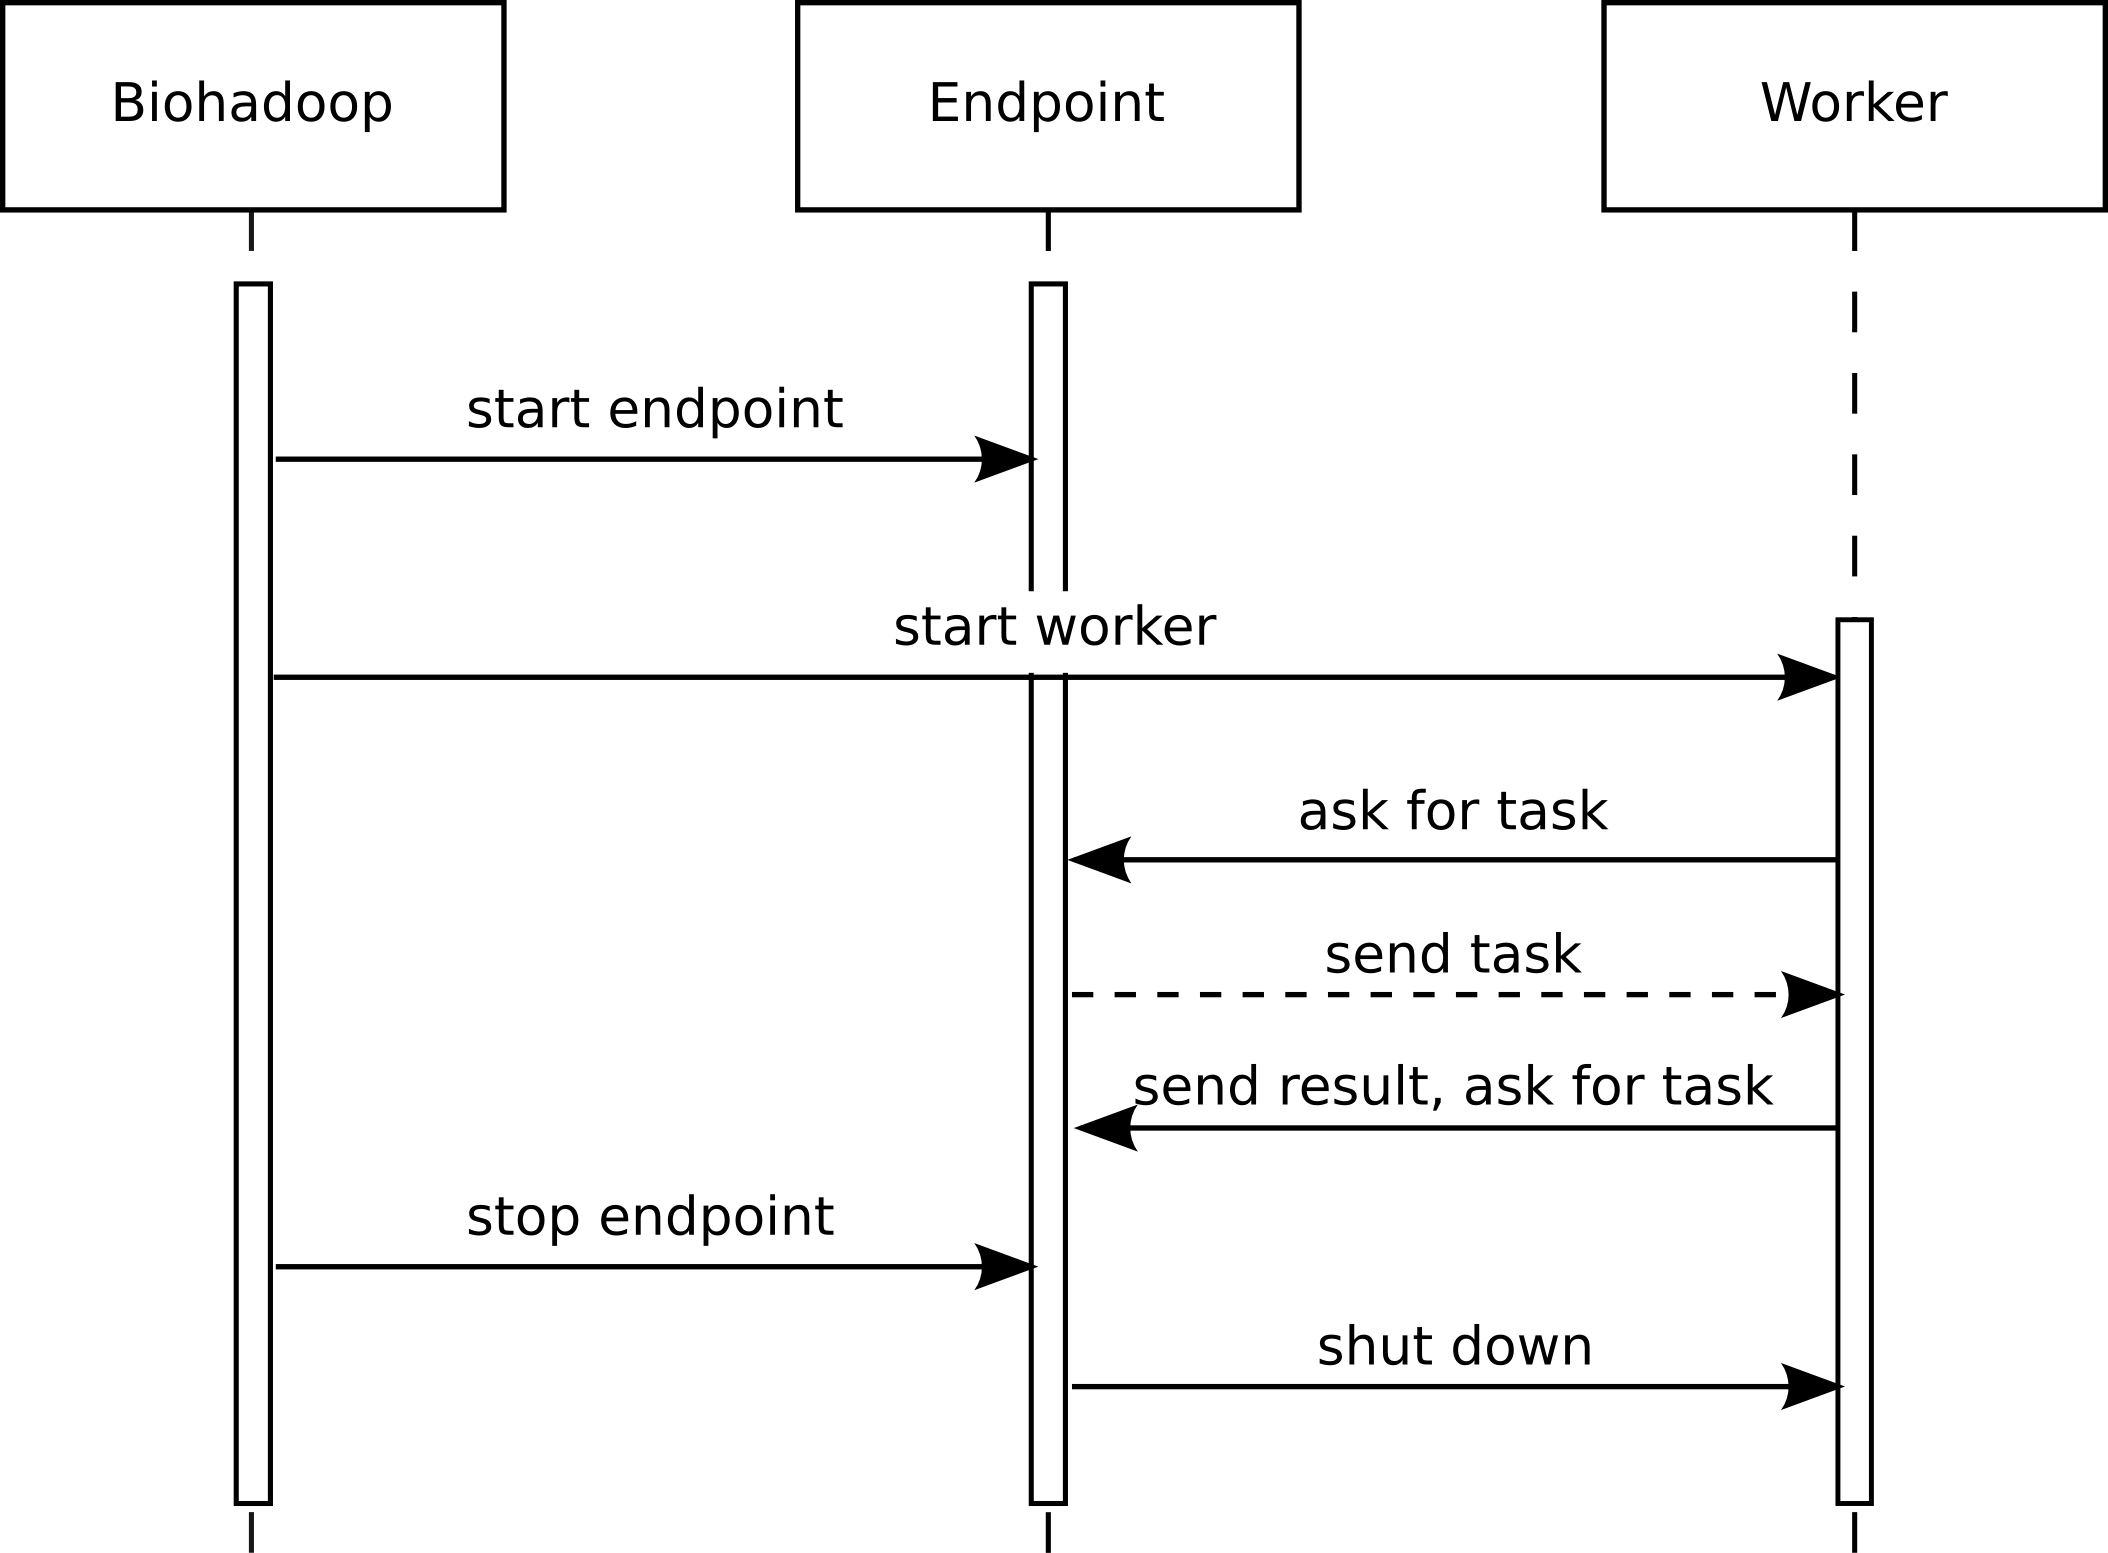
\includegraphics[width=130mm]{flow-worker.png}
%     \caption{Life cycle of a worker}
%     \label{fig:flow-worker}
%   \end{figure}
%   
%   The typical life cycle of a worker is depicted in figure \ref{fig:flow-worker}. It begins at the Biohadoop instance, where the \texttt{buildLaunchArguments(\newline WorkerConfiguration)} method is called to get the necessary parameters. After that, Biohadoop launches for every worker instance a YARN container and starts the \texttt{at.ac.uibk.dps.biohadoop.tasksystem.worker.WorkerStarter} inside it. The \texttt{WorkerStarter} is responsible to call the \texttt{configure(String[] args)} and \texttt{start()} method of the worker. If an exception occurs, it is the responsibility of the \texttt{WorkerStarter} to terminate the work and return a corresponding exit value to Biohadoop. Please note, that figure \ref{fig:flow-worker} lacks information about the steps that are necessary to instrument the adapters. Information about those steps can be found in section \ref{chap:impl:adapter}.
%   
%   Inside the workers \texttt{start()} method, there is a main loop, where the worker asks for new tasks and submits the results of the computation to the adapters, which return them to the algorithm. The workers then wait for new tasks or for a shut down information from the adapters, which leads to its termination.
% 
%   By making the workers actively ask for new work, the adapters don't have to keep track of the workers. This way, the number of workers has no real limit. As long as a worker is able to connect to a corresponding adapter (where they have to agree on the protocol, communication flow and exchanged data, see section \ref{chap:impl:communication-flow} for more information), it may ask for work and return its results.
%   
%   !!!provide and describe implementation for AsyncComputable for Sum algorithm!!!
% 
%   \subsection{AsyncComputable}
%   \label{chap:impl:async-computable}
%   In the previous sections, the task system was introduced, but it wasn't mentioned, how the results for submitted tasks are computed. This is done, by defining classes that implement the generic interface \path{at.ac.uibk.dps.biohadoop.tasksystem.AsyncComputable<R, T, S>}. Each class that implements this interface declares, that it can be executed by workers. When an algorithm submits a new task, it has to define which \texttt{AsyncComputable} should be used for computing the result for the task. This information is then send, along with the task itself, to a worker, where the result is computed and then returned.
%   
%   In listing \ref{listing:asyncComputable-interface}, the method for the \texttt{AsyncComputable} interface is shown, where R is the type of the \texttt{initalData}, T is the type of input data and S is the type of the result.
%   
%   \lstinputlisting[caption=Classes that implement the AsyncComputable interface can be executed by workers,label=listing:asyncComputable-interface]{../listings/chap4-asyncComputable-interface.lst}
%   
%   \begin{itemize}
%     \item \texttt{S compute(T data, R initialData) throws ComputeException}: The code inside this method is executed by the worker. It gets \texttt{data} of type T and \texttt{initialData} of type S as arguments. The \texttt{data} represents the data for this task, \texttt{initialData} is some static data that doesn't change over time and that can be therefor cached by the workers, once they received it the first time. When the computation has finished, the result of type S is returned to an adapter and a new task is requested by the worker. The \texttt{compute(T, R)} method may throw a \texttt{ComputeException} at any time, indicating that something went wrong during the computation. This exception is logged by the workers, after that they terminate.
%   \end{itemize}
%   
%   \begin{figure}[ht!]
%     \centering
%     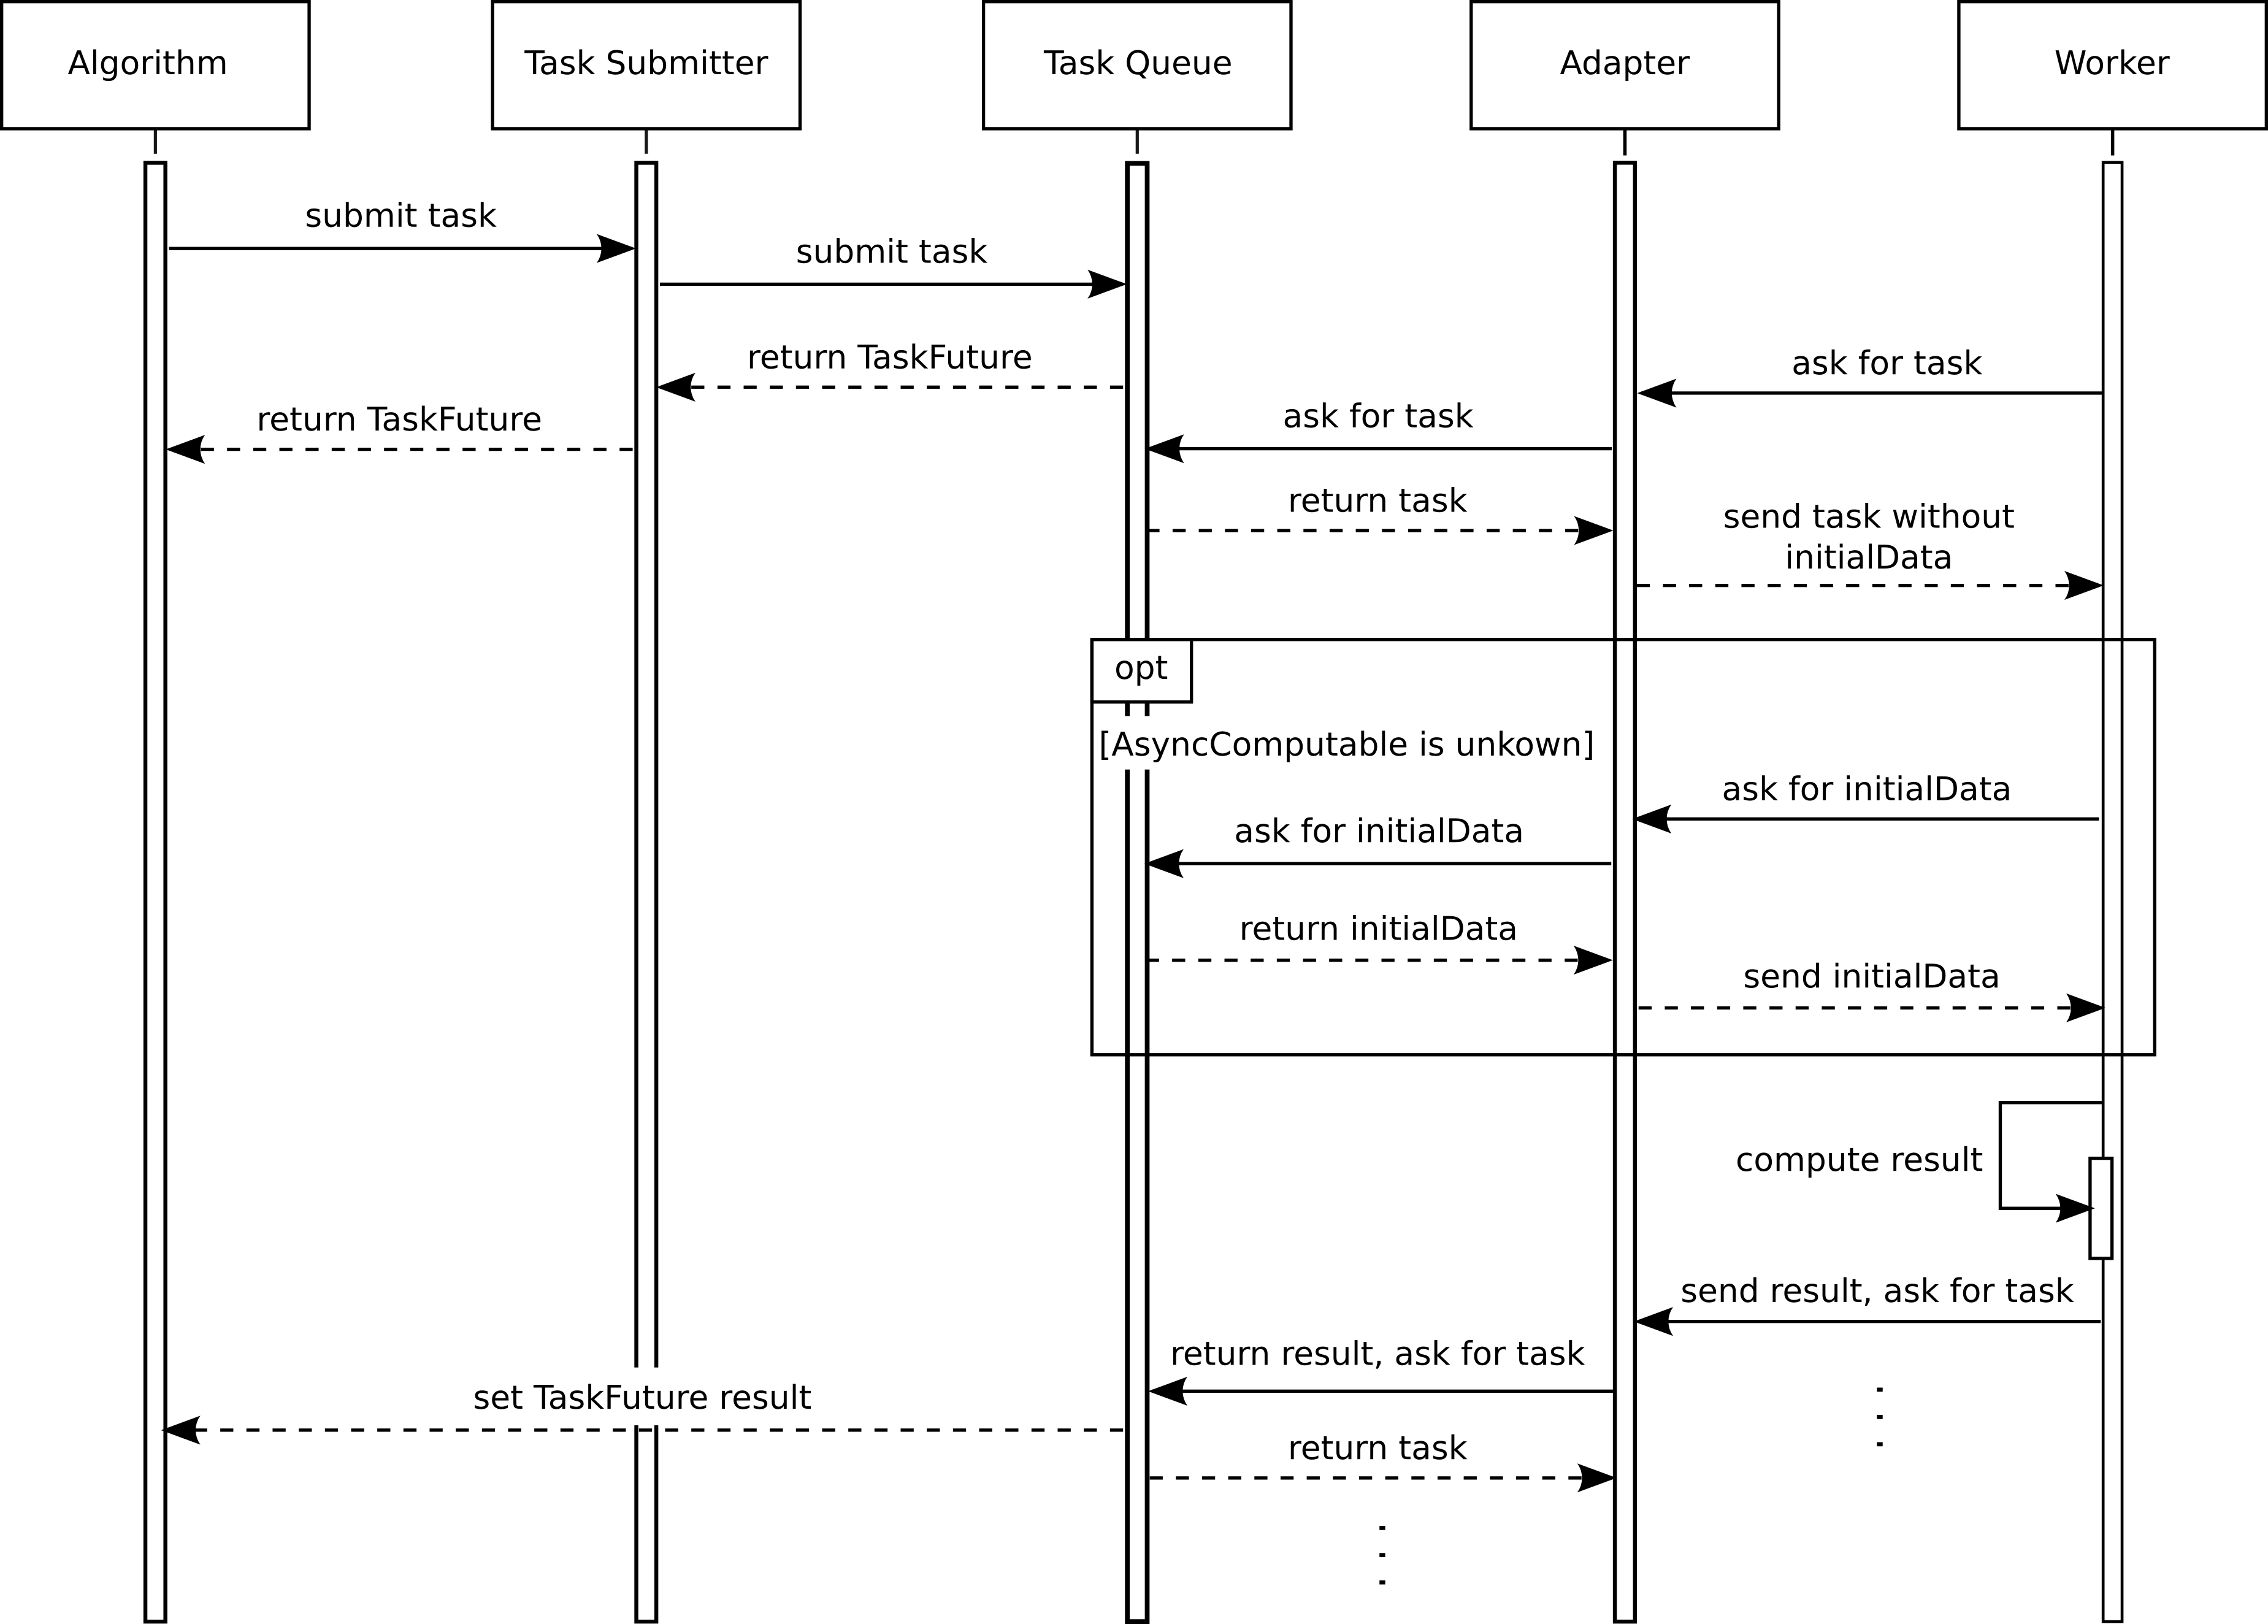
\includegraphics[width=130mm]{flow-asyncComputable.png}
%     \caption{Lifecycle of a task, computed by a worker using an AsyncComputable}
%     \label{fig:async-computable}
%   \end{figure}
%   
%   Figure \ref{fig:async-computable} depicts the general sequence of action for an asynchronous computation: a task is submitted to the task queue by an algorithm. As seen in section \ref{chap:impl:task-submitter}, this should be done using a \texttt{TaskSubmitter}. On submission, an \texttt{AsyncComputable} class must be declared, which is used by workers to compute the result for the task. At some point in time, an adapter takes the task out of the queue, together with the description of its related \texttt{AsyncComputable}. This step is triggered by an incoming worker request. The task, together with the description of its related \texttt{AsyncComputable}, is packed into a message and send to the requesting worker. On the worker side, the message is received and analyzed. Then, the result of the task is computed using an instance of the related \texttt{AsyncComputable}. The result is returned to the adapter and a new task is requested.
%   
%   There is one more step included, if the worker encounters an \texttt{AsyncComputable} that it hasn't seen before. In this case, the worker requests the \texttt{initialData} for this \texttt{AsyncComputable}, and only after it receives this data, it can proceed in computing the result of the task. The \texttt{initialData} should be cached by the worker, to minimize the communication overhead. All worker implementations provided by Biohadoop work this way.
%   
% \section{Communication}
% \label{chap:impl:communication}
%   In Biohadoop, algorithms can take usage of the task system to distribute their computation onto several waiting workers. As seen in the previous chapters, the task system consists of the submitters, a queue, adapters and workers. The submitters, queue and adapters all work in the same JVM and therefor in the same process. The communication between these parts is not difficult, it is just a matter of reading and writing shared variables between the different threads, possibly protected by concurrency protocols (for example, the queue is based on Java's \texttt{LinkedBlockingQueue}, which is a thread safe queue that supports many writers and readers).
%   
%   The communication between the adapters and workers is more complicated, as the adapters and workers may run in different processes, or even on different machines, so they can not rely on sharing variables between some threads. A more sophisticated method of communication must be used.
%   
%   There are many different ways of communication between different (remote) processes. Biohadoop provides five different communication protocols, that can be used to transfer the data between adapters and workers. The reason to not stick to just one implementation was, that each one has its advantages and disadvantages. As the whole communication process is hidden from the algorithm by the task system, changing the communication facility is just a matter of configuration, which makes it easy to try out different protocols and decide later on about which one to use.
%   
%   If there is the need for different, yet not implemented protocols, Biohadoop provides a way to implement its own protocols by implementing the appropriate parts of \texttt{Adapter} (section \ref{chap:impl:adapter}) and \texttt{Worker} (section \ref{chap:impl:worker}). The adapters and workers have to agree about the protocol, the serialization of the data and the communication flow.
%   
%   An introduction to the provided protocols is given in section \ref{chap:impl:protocols}. In section \ref{chap:impl:communication-flow}, the communication flow for the provided protocols is shown. It defines the steps involved for the communication between the adapters and the workers. Those steps are the same for all provided protocols. If one wants to implement its own communication mechanisms, it doesn't have to stick to the presented control flow and is free to choose its own one.
%   
%   \subsection{Protocols}
%   \label{chap:impl:protocols}
%     In this section, the five different communication protocols of Biohadoop are given, each one has its advantages and disadvantages.
% 
%     \subsubsection{HTTP}
%       Biohadoop provides an implementation of adapters and workers, that can communicate to each other by using HTTP. The adapter makes the tasks available as resources under a given URL. The URL is composed by the server name and port where the resource is available and the path \texttt{rs}, which is followed by the name of the task pipeline as subpath. For the default pipeline this would be for example \path{http://example.org/rs/DEFAULT_PIPELINE}. The workers take the tasks from this URL, compute the results and return those results to the same URL by using the \texttt{POST} verb.
%       
%       The main advantage of the HTTP protocol is, that it is in broad usage and that there exists an implementation for it in almost every language. This makes it very easy to write external workers in the desired language. The disadvantage of using HTTP is its speed, as there is a lot of overhead involved when sending HTTP requests over the wire (for example the HTTP headers).
% 
%       For serialization purposes, the JSON format is used. This is a very common format and suitable for machine communication, but also understandable for the human reader. Most programming language support JSON.
%     \subsubsection{Kryo and KryoNet}
%       Kryo \cite{kryo} is a library for high speed serialization of Java objects. It is usually faster than the build-in serialization features of Java. The developers of Kryo provide also the library KryoNet \cite{kryonet} for communication between different remote entities. This library is used by Biohadoop as one type of its provided protocols. The advantage consists of its speed, at least for the serialization.
%       
%       But as there where some problems when using KryoNet, the achieved communication speed is somewhat slower than with most of the other protocols. The problems are related to the asynchronous nature of KryoNet, where all requests are handled by exactly one event loop. If one request blocks (e.g. because it is waiting for new tasks), all other requests block too. To circumvent this, the requests are dispatched to special threads, but this slows the whole system noticeable down.
%       
%       Another disadvantage of Kryo and KryoNet is that they are custom serializers and protocol, that are not in broad usage. This restricts the worker implementations to be written in Java, which may not be a problem at all, especially if only embedded workers are used. But if external workers should be used, they have to be written in Java.
%       
%       Each class, that should be submitted between adapters and workers using Biohadoops Kryo protocol, must be registered with Kryo. The registration can be done by implementing the \path{at.ac.uibk.dps.biohadoop.utils.KryoRegistrator} interface in a registration object. This object then has to be made known to Biohadoop, by specifying its full class name in the \texttt{globalProperties} section of the configuration file (see section \ref{chap:impl:configuration} for more information about this topic). The name of the property must be \texttt{KRYO\_REGISTRATOR}. As an example, lets assume, that the full name of the configurator class is \path{com.biohadoop.KryoConfigurator}, then the property that needs to be set in the \texttt{globalProperties} section would be:
%       \begin{lstlisting}
% "KRYO_REGISTRATOR" : "com.biohadoop.KryoConfigurator"
%       \end{lstlisting}
%       When this parameter is set in the configuration file, Biohadoop knows that the classes, that are listed inside the configurator class, should be registered with Kryo.
%     \subsubsection{Socket}
%       When using the socket protocol, the communication and serialization is performed by the standard Java libraries. The communication is done using sockets, the serialization by the standard Java serializer. Each class, that should be submitted between adapters and workers using the socket protocol, must implement at least the \path{java.io.Serializable} marker interface. This is necessary for the standard Java serialization mechanism to succeed. As this serialization mechanisms can be somehow slow, there is the additional possibility, that a class implements the \path{java.io.Externalizable} interface, where the serialization has to be done manually.
%       
%       The advantage of the socket protocol is its very good performance, and that it is just a plain socket. Most languages provide mechanisms to connect to a socket, so this should be a rather easy task.
%       
%       The disadvantage of Biohadoops socket protocol is its dependence on the Java serialization, which restricts the workers to be written in Java or in a language that provides implementations for the Java serialization. This disadvantage may be mitigated by the possibility to implement a custom serialization mechanism by implementing the \texttt{Externalizable} interface.
%     \subsubsection{WebSocket}
%       WebSockets can be used for bidirectional communication. They were first used as an additional type of communication between a web application and an application server. They rely on the HTTP protocol for the handshake, during which the communication partners agree to upgrade to the WebSocket protocol. After the upgrade is done, the communication between the endpoints (in this case between the adapters and workers) can be performed using binary or text streams. Unlike in the plain HTTP protocol, the HTTP headers are not transmitted with every message, which reduces their size.
%       
%       Like in HTTP, the adapter makes the tasks available as resources under a given URL. The URL is composed by the server name and port where the resource is available, the path \texttt{ws}, which is followed by the name of the task pipeline as subpath. For the default pipeline this would be for example \path{http://example.org/ws/DEFAULT_PIPELINE}
%       
%       Unlike the HTTP protocol, for WebSockets there is no need to make a distinct request for every exchanged message. The worker just connects once to the URL and can then exchange all messages through this established connection.
% 
%       As already mentioned, the HTTP headers are omitted when WebSockets are used. This makes the data transfer faster than with HTTP, which is one of the advantages of using the WebSocket protocol in Biohadoop. Another advantage is, that WebSocket implementations are now available in many programming languages, making them available to a broad range of users, that may implement workers in their desired language. The disadvantage is that, if no WebSocket implementation exists in a language, it is harder to write a client, than e.g. for HTTP. Also, as WebSockets are a relatively new type of communication protocol, some available libraries may still contain bugs.
%       
%       JSON is used as the format for the data serialization, most languages provide parsers for it.
%     \subsubsection{Local}
%       The local communication can only be used with local workers. Those are workers, that run inside the same JVM (and therefor process) as Biohadoop and the algorithms. This makes it very easy to submit tasks and return results between adapters and workers. The data transfer is simply done by accessing shared variables. No serialization is needed, which greatly speeds up the communication between the adapters and workers. The access to the shared variables must be synchronized, as there may be several adapters and workers. This is done through standard Java mechanisms.
%       
%       The main advantage of the local protocol is its speed. As a process may use as much computational resources as available and because current hardware may provide a lot of shared CPU cores, the local protocol and workers may even scale to a sufficient degree for many tasks. But when greater scalability is needed, or when there are not enough computational resources available on the machine that runs Biohadoop, remote workers are needed, that rely on other communication protocols than the local one. Therefor the biggest disadvantage of local workers is, that they can run only on the local machine, where also Biohadoop runs.
%       
%   \subsection{Communication flow}
%   \label{chap:impl:communication-flow}
%     Each protocol presented in the prior section has to use some kind of communication flow between the corresponding adapters and workers. This communication flow, depicted in figure \ref{fig:communication-flow} is the same for all protocols that are provided by Biohadoop. If one wants to write a worker for one of the provided protocols, it must adhere to the communication flow presented here. Custom protocols don't need to reuse this, they are free to implement their own communication pattern.
%     
%     \begin{figure}[ht!]
%       \centering
%       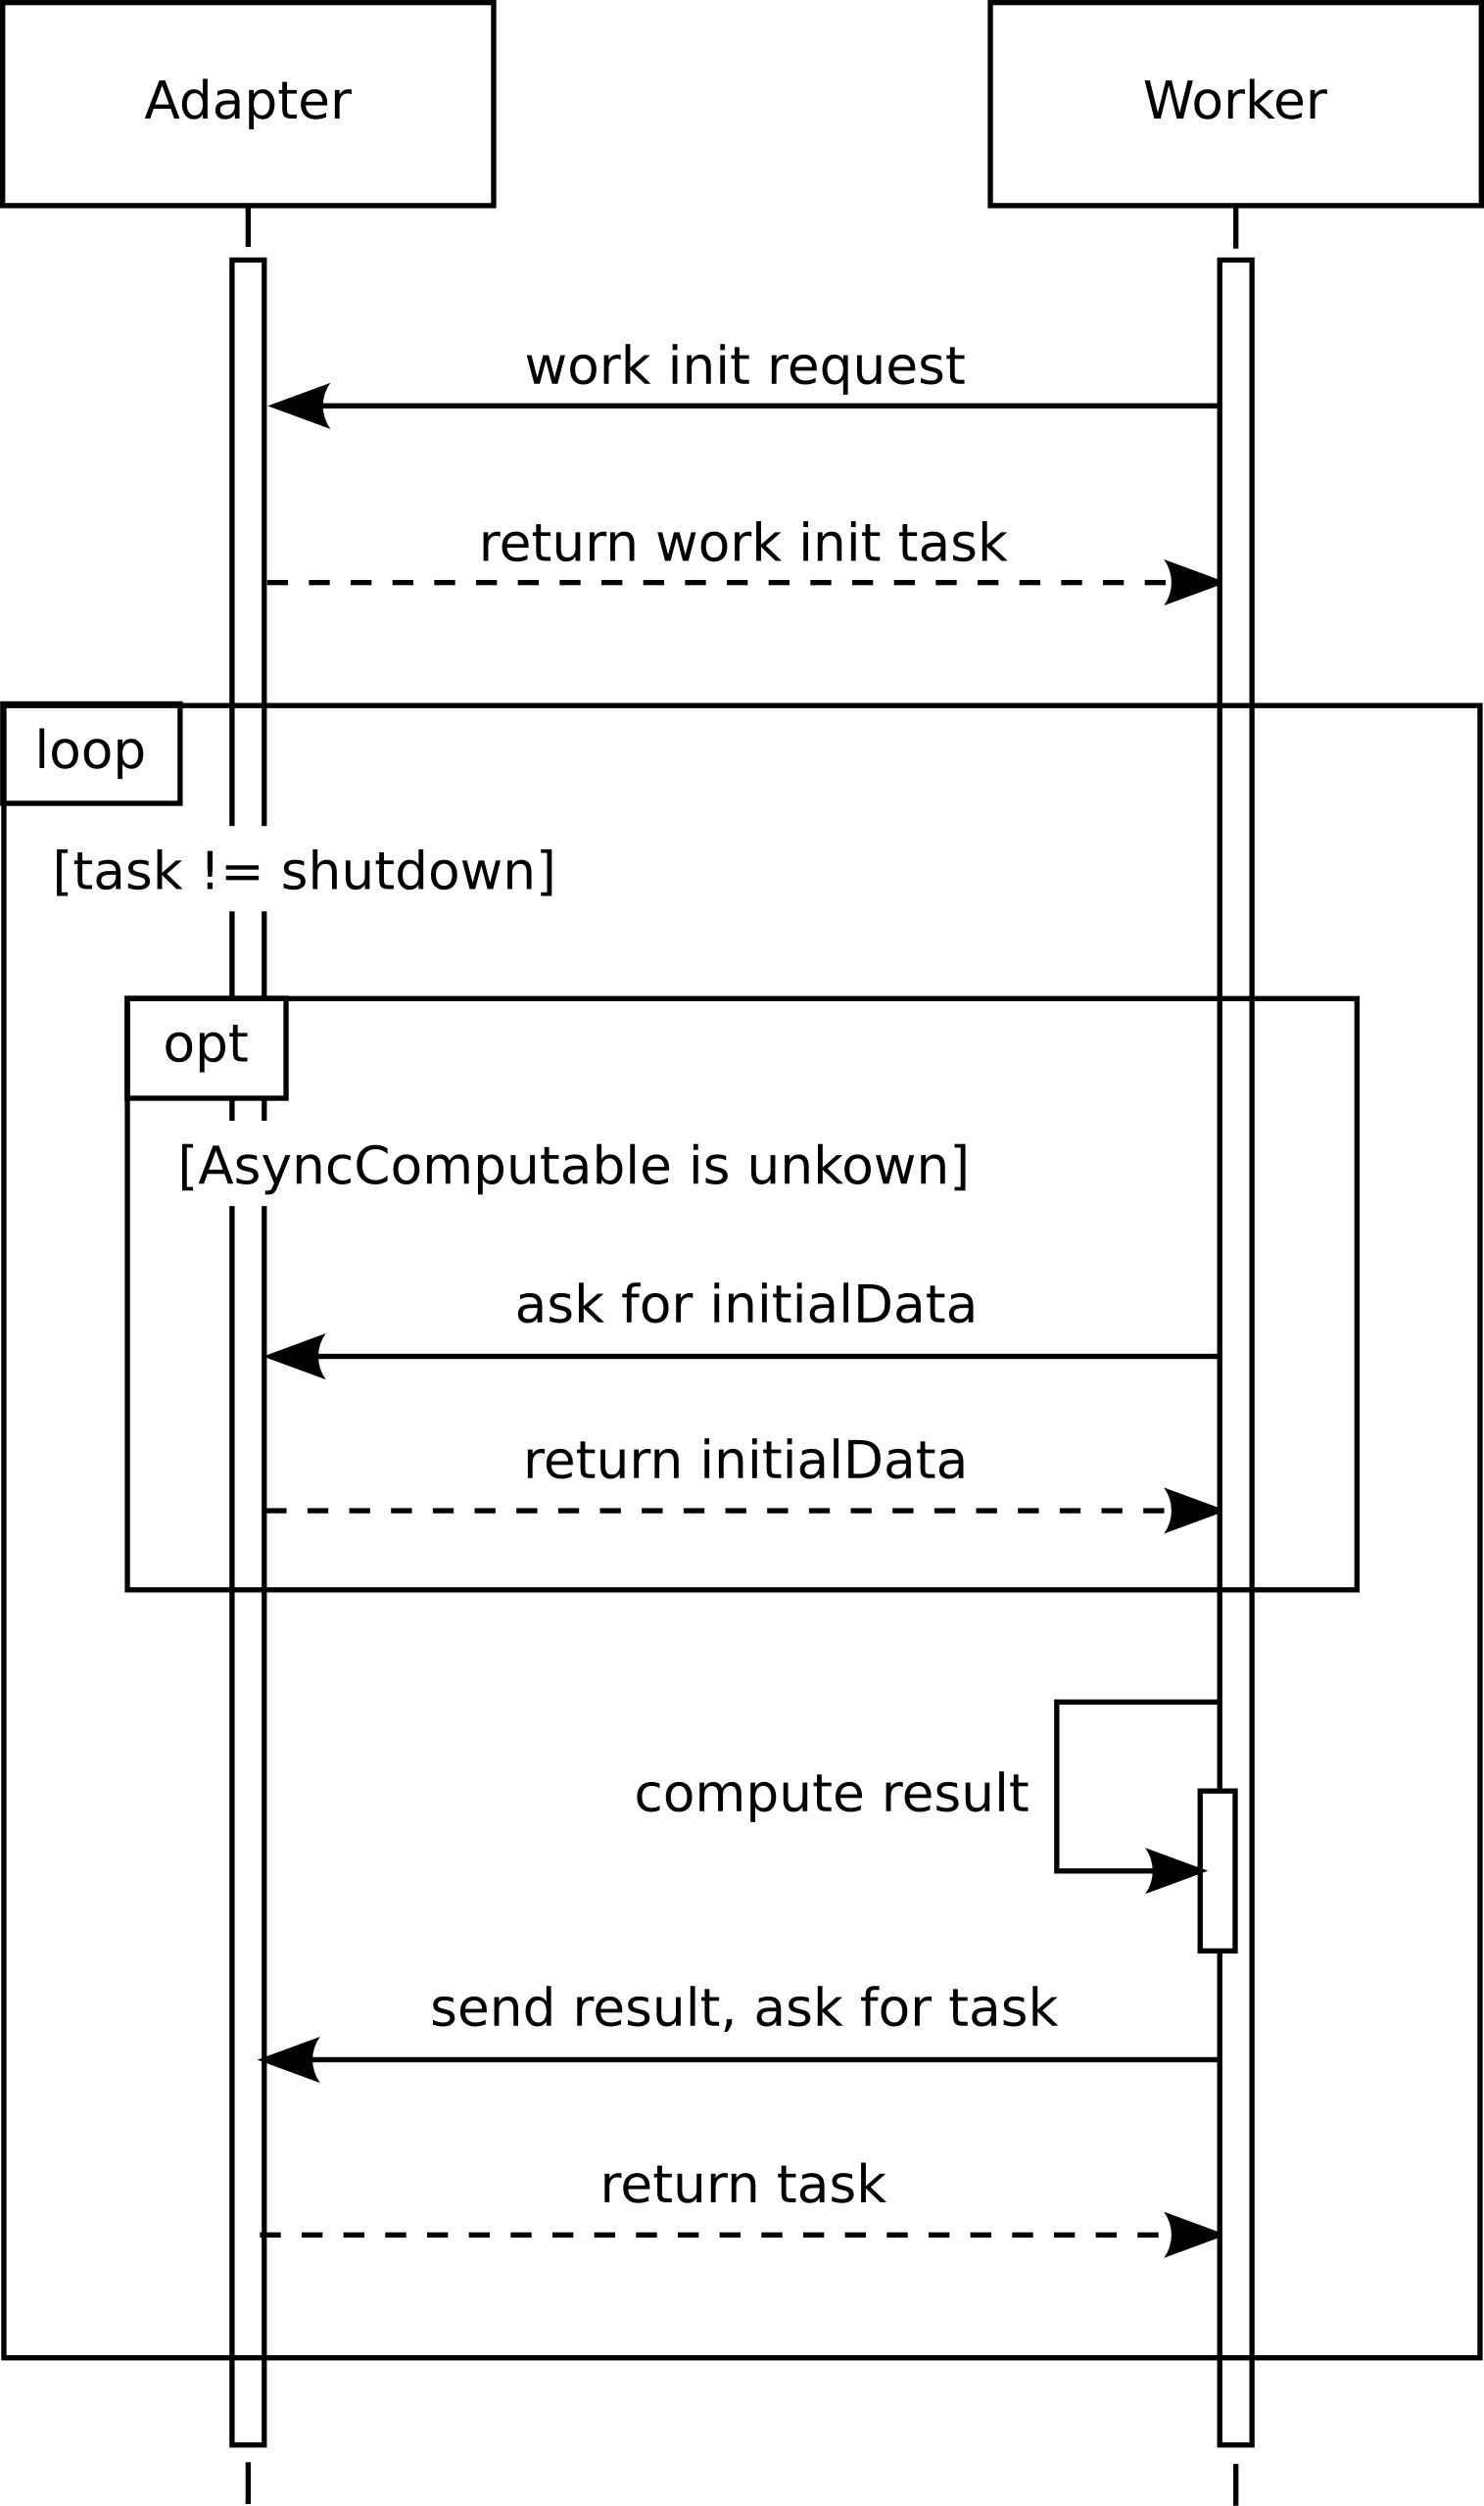
\includegraphics[width=100mm]{communication-flow.png}
%       \caption{Communication flow}
%       \label{fig:communication-flow}
%     \end{figure}
%     
%     As one can see in figure \ref{fig:communication-flow}, the communication between adapters and workers is initialized by the worker. Also, after each iteration, the worker actively asks for new tasks.
%     
%     After the worker gets a task from the adapter, it has to control, if it already has the needed \texttt{initialData}. This is done by looking at the class name of the \texttt{AsyncComputable}, which is send along with the task. If the class is unknown, the worker asks the adapter for the \texttt{initialData} for the task. The adapter responds with the \texttt{initialData}, that is then cached by the worker, in case that the result for another task with the same \texttt{AsyncComputable} should be computed. Then, the worker computes the result for the task using the tasks data, the \texttt{AsyncComputable} and the \texttt{initialData}. The result is then retransmitted to the adapter and, at the same time, a new task is requested. Then the loop starts from the beginning.
%     
%     If the answer of the adapter consists of a shutdown message, the worker disconnects from the adapter and does the shutdown.
%     
%     The implementation of the presented communication flow has one big problem: a worker doesn't recognize when the same  \texttt{AsyncComputable} is used for different kinds of tasks with different \texttt{initialData} values. For example, lets assume that we have two different tasks, \texttt{TASK\_A} and \texttt{TASK\_B}. Each task uses the same \texttt{AsyncComputable} for its computation, but a different \texttt{initialData} value. Lets further assume, that a worker first encounters \texttt{TASK\_A}. In this moment, the worker will look up internally, if it has already the \texttt{initialData} for the \texttt{AsyncComputable}, that comes along with the task. In this case, this is not true, as the worker encounters this \texttt{AsyncComputable} the first time. The worker asks the adapter for the \texttt{initialData} and after its retrieval it stores this data internally. Then it computes the result for the task and returns it to the adapter. Now lets assume, that the worker gets next the \texttt{TASK\_B}. As the \texttt{AsyncComputable} is the same as for \texttt{TASK\_A}, and the worker looks up the \texttt{initialData} based on the \texttt{AsyncComputable}, the worker believes that it knows already the right \texttt{initialData}, which is wrong.
%     
%     This problem can be solved by transmitting a hash value of the \texttt{AsyncComputable} and \texttt{initialData}, in addition to the normal task data, and letting the worker decide, based on this hash, if it needs to fetch the \texttt{initialData}. This is not a big code change, and is on top of the TODO list for Biohadoop.
% 
% \section{Enhancements}
% \label{chap:impl:enhancements}
%   Beside the task system, that is presented in greater detail in section \ref{chap:impl:task-system}, Biohadoop provides two enhancements for algorithm authors. One is about persistence, where it is possible to load and store some data to disk (see section \ref{chap:impl:persistence}). The other is about high level parallelism between parallel running algorithms, called the ``iceland model'', that is sometimes used by optimization algorithms to enhance the solution (see section \ref{chap:impl:island-model}).
% 
%   \subsection{Persistence}
%   \label{chap:impl:persistence}
%   There are a lot of reasons for an algorithm to store its data to a disk. The most important may be, that one wants to store the result of a computation. The next reason is, to store the computational work that is done until a certain point, in case something happens. If this data can be reloaded afterwards, the computation can be continued from that point on. Another reason may be, that the intermediate results are needed for some other computation or visualization.
%   
%   So we see, that some kind of persistence is useful. It should include both the saving and loading of data. Biohadoop provides this kind of service by offering a simple API. Of course, an algorithm author may opt to use its own mechanism of data storage and retrieval, but the presented API has the advantage, that it is able to run both on local file systems and on Hadoops HDFS.
%   
%   The file saving is performed by using the class \path{at.ac.uibk.dps.biohadoop.persistence.FileSaver} and its provided static method, as presented in listing \ref{listing:chap4-persistence-save}.
%   
%   \lstinputlisting[caption=Save method exposed by \texttt{FileSaver},label=listing:chap4-persistence-save]{../listings/chap4-persistence-save.lst}
%   
%   \begin{itemize}
%     \item \texttt{static void save(SolverId solverId, Map<String, String>\newline properties, SolverData<?> solverData) throws\newline FileSaveException}: This method saves the data, provided by the \texttt{solverData} argument, to a file. The path for the file consists of the path that is defined in the configuration file under the algorithms private property with name \texttt{FILE\_SAVE\_PATH}, enhanced with the \texttt{solverId}. The filename consists again of the \texttt{solverId}, the iteration count that is submitted through the \texttt{SolverData} and the timestamp, at which the saving is done. The elements of the filename are separated by the character \texttt{\_}.
%     
%     So, for example, lets assume that the path defined in the configuration file is \path{/biohadoop/save}, the unique \texttt{solverId} is a UUID and has the value \path{08b1bc4c-e6d9-44ec-ba5d-24801f6c2339}, the iteration count is \text{100} and the timestamp, at which the saving is done, has the value \texttt{1411588421915}. Then the data, submitted with the \texttt{solverData} argument, is saved in the file:   
%     \begin{lstlisting}
% /biohadoop/save/08b1bc4c-e6d9-44ec-ba5d-24801f6c2339/08b1bc4c-e6d9-44ec-ba5d-24801f6c2339_100_1411588421915
%     \end{lstlisting}
%     
%     The saved data is stored in the file using the JSON format, which is a nice format for data serialization, that is available in many different programs, programming languages and environments.
%     
%     The method \texttt{save(SolverId, Map<String, String>, SolverData<?>)} throws a \texttt{FileSaveException} in the following cases:
%     \begin{itemize}
%       \item the \texttt{FILE\_SAVE\_PATH} property is not set
%       \item the save path can not be created
%       \item a file with the given name already exists
%       \item there was an error during the save operation
%     \end{itemize}
%     It is the responsibility of the algorithm author, to act appropriately to such an exception.
%   \end{itemize}
%   
%   As mentioned, the saving is configured in the configuration file. There are two properties, by which the saving can be adjusted to the personal needs (for more information about the configuration of Biohadoop, refer to section \ref{chap:impl:configuration}):
%   \begin{itemize}
%     \item FILE\_SAVE\_PATH: This is the initial path, where the files should be stored when they are saved. See the description of the \texttt{save(SolverId, Map<String, String>, SolverData<?>)} method above for more information about how the final file name is defined.
%     \item FILE\_SAVE\_AFTER\_ITERATION: Through this property, an algorithm author can decide after how many iterations a file should be saved. This removes from the algorithm author the burden of checking the iteration by hand. The \texttt{save} method than compares this value with the value that is provided in the \texttt{solverId} argument and decides, if it should persist the data.
%   \end{itemize}
%   
%   To load a file, for example to resume an old computation at the beginning of an algorithm, the class \path{at.ac.uibk.dps.biohadoop.persistence.FileLoader} can be used. This class provides a static method, presented in listing \ref{listing:chap4-persistence-load}.
%   
%   \lstinputlisting[caption=Load method exposed by \texttt{FileLoader},label=listing:chap4-persistence-load]{../listings/chap4-persistence-load.lst}
%   
%   \begin{itemize}
%     \item \texttt{static SolverData<?> load(SolverId solverId, Map<String, String>\newline properties) throws FileLoadException}: This method loads data from a file that is defined in the private property section of the algorithm under the name \texttt{FILE\_LOAD\_PATH}. This value can be defined in two ways. The first one defines the full path for a file, including the file name, that contains loadable data in a JSON format. In this case, exactly this file is loaded. In the second case, the value defines a directory path where loadable files can be found. In this case, the latest file in the directory is loaded, which is the file that was modified most recently. This can be suitable, when always the newest file of a directory should be loaded.
%     
%     The method throws a \texttt{FileLoadException} in the following cases:
%     \begin{itemize}
%       \item the \texttt{FILE\_LOAD\_PATH} property is not set
%       \item the file or path can not be found
%       \item the \texttt{FILE\_LOAD\_PATH} points to an empty directory
%       \item there was an error during the save operation
%     \end{itemize}
%     It is the responsibility of the algorithm author, to act appropriately to such an exception.
%   \end{itemize}
% 
%   Like in the case of file saving, the loading is configured in the configuration file. There are two properties, by which the loading can be adjusted to the personal needs:
%   \begin{itemize}
%     \item FILE\_LOAD\_PATH: This is the initial path, where the files should be stored when they are saved. See the description of the \texttt{save(SolverId, Map<String, String>, SolverData<?>)} method above for more information about how the final file name is defined.
%     \item FILE\_LOAD\_ON\_STARTUP: This boolean property defines, if the configured file should be loaded at all (the name is a bit confusing). If this property is not set, a call to \texttt{load} returns null as result. This can be convenient, if there is no useful data to load.
%   \end{itemize}
%   
%   \subsection{The island model}
%   \label{chap:impl:island-model}
%   The island model is a high level parallelization model, that is sometimes used in optimization problems. In the island model, there are several optimization algorithms running in parallel, trying to compute the result to the same problem. Those optimizers are called the islands. Each of these optimizers is independent of the others, and each one may have a different solution at a given point of time. By exchanging their data after some intervals, islands may get interesting solutions from other islands, that can be integrated in their own computation to enhance their solution.
%   
%   The island model greatly enhances the exploration behavior of optimizers, which often results in better overall solutions. As the data exchange is only done at certain points of time, the optimizers have the chance to exploit their own solution. When they get stuck in a local optima, they get the chance to escape this optima by getting another solution from another island.
%   
%     \subsubsection{API}
%     \label{chap:impl:island-model-api}
%     Biohadoop provides an API that can be used to build an island model. This API is exposed through the class \path{at.ac.uibk.dps.biohadoop.islandmodel.IslandModel} as seen in listing  \ref{listing:chap4-island-model}.
%     
%     \lstinputlisting[caption=Methods exposed by the \texttt{IslandModel} class. The class can be used to exchange data between the islands and therefor to construct an island model,label=listing:chap4-island-model]{../listings/chap4-island-model.lst}  
%     
%     \begin{itemize}
%       \item \texttt{static void initialize(SolverId solverId) throws\newline IslandModelException}: This method must be called by an algorithm to register it at the ZooKeeper service (see below for more information about ZooKeeper). It takes the \texttt{solutionId} as its only argument, which is the unique identifier for the algorithm.
%       
%       The method throws a \texttt{IslandModelException} if the host or port of ZooKeeper is not specified in the global properties of the configuration file. The host is specified through the \texttt{ZOOKEEPER\_HOSTNAME} property, the port through the \texttt{ZOOKEEPER\_PORT} property.
%       \item \texttt{static Object merge(SolverId solverId, Map<String, String>\newline properties, SolverData<?> solverData) throws\newline IslandModelException}: This method should be called, when the data merging should be done. The \texttt{solverId} identifies the algorithm, the \texttt{solverData} contains the current solution.
%       
%       The properties object is the map configured in the private property part of the algorithm. It uses strings for the keys and the values and must contain the following properties:
%       \begin{itemize}
% 	\item \texttt{ISLAND\_DATA\_REMOTE\_RESULT\_GETTER}: This property specifies a class that implements the interface \path{at.ac.uibk.dps.biohadoop.islandmodel.RemoteResultGetter} with the following method:
% 	\begin{lstlisting}
% Object getBestRemoteResult(List<NodeData> nodesData) throws IslandModelException
% 	\end{lstlisting}
% 	It has the job to get an appropriate remote result from a remote island. To perform this job, a list of \texttt{NodeData} elements is provided, that represents all currently known islands. From this list, a suitable solution should be chosen and returned.
% 	\item \texttt{ISLAND\_DATA\_MERGER}: This property specifies a class that implements the merging of the local and a remote solution. This class must implement the generic \path{at.ac.uibk.dps.biohadoop.islandmodel.DataMerger} interface with the following method, where T is the generic type:
% 	\begin{lstlisting}
% T merge(T o1, T o2)
% 	\end{lstlisting}      
% 	The job of this method is to merge the data of the solutions given as \texttt{o1} and \texttt{o2} into a new solution.
%       \end{itemize}
%       
%       The \texttt{merge(SolverId, Map<String, String>, SolverData<?>)} method throws an \texttt{IslandModelException} at the same conditions as the \texttt{initialize(SolverId)} method mentioned above. In addition, it throws the \texttt{IslandModelException} if the \texttt{RemoteResultGetter} or the \texttt{DataMerger} classes are not defined or can not be instantiated. Also, the \texttt{RemoteResultGetter} or the \texttt{DataMerger} may throw this exception, if there is something wrong during the data merging. It is the responsibility of the algorithm author, to act appropriately to such an exception.
%     \end{itemize}
%     
%     To make its own solution available to other islands, the data must be explicitly set by the algorithm author. This is done by using the following method of the \path{at.ac.uibk.dps.biohadoop.datastore.DataClient} object:
%     \begin{lstlisting}
% static <T> void setData(SolverId solverId, Option<T> option, T data)
%     \end{lstlisting}   
%     
%     It takes as arguments the \texttt{solverId}, the second argument in this case must be \path{DataOptions.SOLVER_DATA}, and the third argument should be the data, wrapped in a \path{at.ac.uibk.dps.biohadoop.solver.SolverData} object.
% 
%     \subsubsection{ZooKeeper}
%     \label{chap:impl:island-model-zookeeper}
%     As mentioned above, Biohadoops island model API takes usage of ZooKeeper \cite{zookeeper}, which is a Server that provides distributed configuration and synchronization services, and a naming registry. Therefor, a running ZooKeeper instance must be accessible by Biohadoop.
%     
%     When using the island model, the algorithms first have to register to ZooKeeper by using the \texttt{initialize(SolverId)} method of the \texttt{IslandModel}. The registration adds an entry to ZooKeeper, that is visible to all other algorithms that use the island model API. The path to the registration is defined by the fixed string \path{/biohadoop/solvers}, followed by the simple class name of the algorithm and the \texttt{solverId} as subpath. For example lets assume that the full class name of our algorithm is \path{org.example.Sum} and that its \texttt{solverId} is \texttt{08b1bc4c-e6d9-44ec-ba5d-24801f6c2339}. Then the path, at which the algorithm registers itself to ZooKeeper is
%     \begin{lstlisting}
% /biohadoop/solvers/Sum/08b1bc4c-e6d9-44ec-ba5d-24801f6c2339
%     \end{lstlisting}
%     
%     The registration data consists, again, of the \texttt{solverId} and a URL, where the current solution for the algorithm can be found, both serialized using the JSON format. An example for this data can be found in listing \ref{listing:chap4-zookeeper-registration-data}, where the relevant information is on line 1.
%     
%     \lstinputlisting[caption=Example for ZooKeeper registration data,label=listing:chap4-zookeeper-registration-data]{../listings/chap4-zookeeper-registration-data.lst}
%       
%     When the data merging between islands should be done, the defined \texttt{RemoteResultGetter} gets a list of all the algorithms that are registered at ZooKeeper, along with their registration data. With this information, that contains also the URL where the current solution for the islands can be found, the \texttt{RemoteResultGetter} chooses which remote solution should be used for the subsequent merge.
%     
%     The remote solutions are made available as HTTP resources at the URL that is part of the registration information, where the complete URL consists of the URL from the ZooKeeper registration with the \texttt{solverId} appended, for example:
%     
%     \begin{lstlisting}
% http://example.org:30000/rs/islandmodel/08b1bc4c-e6d9-44ec-ba5d-24801f6c2339
%     \end{lstlisting}  
%     
%     In the end, the whole process of registration to ZooKeeper, retrieval of this information from ZooKeeper and publishing the result of the computation at a defined URL is done by the island model API behind the curtains, so an algorithm author doesn't have to bother with it. The only things an algorithm author has to do is to
%     \begin{itemize}
%       \item provide its data using the \texttt{DataClient.setData(SolverId, Option<T>, T)} method
%       \item use the provided methods of the \texttt{IslandModel} object when the merging should be done
%       \item provide an implementation of \texttt{RemoteResultGetter} and \texttt{DataMerger} to define which data should be merged and how the merging should be done
%     \end{itemize}
% 
%     By using ZooKeeper as central registry for the island model, and by exchanging the data between the islands through HTTP, it doesn't matter if the algorithms run in the same Biohadoop instance (which is possible by defining several instances in Biohadoops configuration file), or if the algorithms run in different Biohadoop instances. The only advantage of running several algorithms in the same Biohadoop instance is, that it guarantees that they all run at the same time. When running several Biohadoop instances on Hadoop, it isn't guaranteed that they also run at the same time, as Hadoop decides when to launch a program. If the algorithms don't run at the same time, then there is no data exchange possible between them, so the island model is reduced to one single island, which means that it makes no difference to running the algorithm without the island model.
%   
% \section{Configuration}
% \label{chap:impl:configuration}
%   Biohadoop uses a configuration file in JSON format. This has the advantage, that it isn't hard for humans to understand and modify its content. It usually is also smaller in size than e.g. XML and parsers exist for a broad range of programming languages. To provide support for automatic schema validation, JSON Schema \cite{json-schema} is used. The full JSON Schema \cite{json-schema} for the configuration file can be found in the appendix \ref{lst:json-schema}.
%   
%   The path to the configuration file must be given on invocation of Biohadoop as its first parameter (more information on how to run Biohadoop can be found in \ref{chap:usage:run}). If the path is empty or wrong, Biohadoop stops immediately with an \texttt{IllegalArgumentException}. If a file is found, its content is parsed and Biohadoop tries to build a configuration object out of it. If there was an error during parsing, Biohadoop stops with an \texttt{IOException}, \texttt{JsonParseException} or \texttt{JsonMappingException}, depending on the reason of the error. Supposing everything went right, the configuration is exposed through the static class \path{at.ac.uibk.dps.biohadoop.hadoop.Environment} and its \texttt{getBiohadoopConfiguration()} method.
%   
%   Note that the exposure is restricted to the JVM that runs Biohadoop. But this should be enough for most purposes. The algorithms can directly access the \texttt{Environment}, although this should be seldom necessary, as the algorithm get their parameters as arguments. Adapters are also able to access the \texttt{Environment}. Both mentioned components run in the same JVM as Biohadoop does.
%   
%   When it comes to the workers and the \texttt{AsyncComputable} methods that they run, things are a little bit different. The workers run on different JVMs than Biohadoop does (except the local running workers, that run as separate threads), so they don't have direct access to the \texttt{Environment} object. Nevertheless, the path to the configuration file is provided also to the workers, such that they could read and parse the configuration file. But at the time of this writing, there was no reason for a worker or \texttt{AsyncComputable} to access the configuration file directly, therefor the access is currently not implemented. Changing this at a later stage is not a big task.
%   
%   The configuration file itself consists of the following four top-level objects:
%   \begin{itemize}
%     \item \texttt{communicationConfiguration}: defines lists for additional adapters and all workers, that Biohadoop should start. Additional in the sense, that adapters for dedicated pipelines must be configured right here, whereas adapters for the default pipeline don't have to be configured. The workers must be also defined here, for all pipelines including the default pipeline, since there is no useful default configuration for workers. 
%     \begin{itemize}
%        \item \texttt{dedicatedAdapters}: a list of additional adapters. Each element in the list is of type \path{at.ac.uibk.dps.biohadoop.tasksystem.adapter.AdapterConfiguration}, that contains the canonical class name of an \texttt{Adapter} and a string that defines to which pipeline that adapter belongs.
%        \begin{itemize}
%          \item \texttt{adapter}: canonical class name of the \texttt{Adapter}
%          \item \texttt{pipelineName}: string that defines to which pipeline that adapter belongs
%        \end{itemize}
%        \item \texttt{workerConfigurations}: a list of workers: Each element in the worker list is of type \path{at.ac.uibk.dps.biohadoop.tasksystem.worker.WorkerConfiguration}, that contains the canonical class name of a \texttt{Worker}, a string that defines to which pipeline that worker belongs and a counter that indicates how many instances of this worker should be started.
%        \begin{itemize}
%          \item \texttt{worker}: canonical class name of the \texttt{Worker}
%          \item \texttt{pipelineName}: string that defines to which pipeline that worker belongs
%          \item \texttt{count}: number of instances of this worker
%        \end{itemize}
%     \end{itemize}
%     \item \texttt{globalProperties}: a map with strings as keys and values. This properties are used for global settings, that should be available in different places.
%     \item \texttt{includePaths}: a list of strings that define the paths where needed libraries can be found. This isn't important for a local running instance of Biohadoop (e.g. during development), as the necessary classpaths must be set when starting Biohadoop. But it is important when Biohadoop runs in the Hadoop environment, as this are the paths with libraries, that Hadoop should provide to Biohadoop when running. If the paths to the necessary libraries are not set correctly when running on Hadoop, \texttt{ClassNotFoundException} are thrown.
%     \item \texttt{solverConfiguration}: a list of algorithms that should be run by Biohadoop. Each element in the list is of type \path{at.ac.uibk.dps.biohadoop.solver.SolverConfiguration}, that contains the canonical class name of an \texttt{Algorithm}, a freely selectable name for it, and a map of properties, that are passed to the algorithm as argument.
%     \begin{itemize}
%       \item \texttt{algorithm}: canonical class name of the \texttt{Algorithm}
%       \item \texttt{name}: freely selectable name, is shown for example in the log files
%       \item \texttt{properties}: a map with strings as keys and values. This properties are used for this instance of the algorithm and should be considered private to it. This properties are provided as second argument to the algorithm, when its \texttt{compute(SolverId, Map<String, String>)} method is invoked.
%     \end{itemize}
%   \end{itemize}
% 
%   Listing \ref{lst:sum-configuration} illustrates a very simple configuration file for the \texttt{Sum} algorithm, introduced in section \ref{chap:impl:system-architecture}. The implementation can be found in \cite{biohadoop-algorithms}. The algorithm sums up all values of an integer array. It takes as input arguments the the number of chunks (\texttt{CHUNCKS}) of integer arrays. As second input argument it takes the size of each chunk (\texttt{CHUNCK\_SIZE}). The whole integer array has then the size $\texttt{CHUNCKS} * \texttt{CHUNCK\_SIZE}$. The chunks are submitted to the task system, the sum for each chunk is computed on workers and then returned back to the algorithm, where the final summation for all chunks is done.
% 
%   \lstinputlisting[caption=Simple configuration file for the \texttt{Sum} algorithm\, introduced in section \ref{chap:impl:system-architecture},label=lst:sum-configuration]{../listings/chap4-sum-configuration.lst}
%   
%   At line 2 we have the configuration of the paths, that have to be included when running Biohadoop. This setting is only important if Biohadoop runs in a Hadoop environment. It is not important if it runs in local mode, for example during development. When running on Hadoop, the files in this directories are made available to Biohadoop.
%   
%   At line 3 starts the communication configuration, which consists of a list of dedicated adapters and a list of all workers. The definition of dedicated adapters at line 4 is empty, as \texttt{Sum} uses only the default pipeline for computation. If dedicated pipelines were used, than the adapters for this pipeline must be configured here.
%   
%   Beginning with line 5 we have the declaration of the workers, that Biohadoop should launch. Each entry is defined by the a worker class name, a pipeline to which this worker is assigned, and the number of workers of this instance, that should be launched. We see here for example, that 5 workers of different types are configured, but only the \texttt{LocalWorker} at line 10 should be instantiated once. All other workers have a count of 0, which means that no instances of these workers are launched.
%   
%   At line 27 we have the definition of the global properties. Again, \texttt{Sum} doesn't take usage of this configuration possibility. Other algorithms instead use this place for example to specify the configuration for ZooKeeper.
%   
%   At line 28, the definition for the algorithm starts. In this case, only one algorithm should be started, it is the algorithm with class \texttt{SumAlgorithm}. The name of the algorithm is \texttt{SUM}, which can be seen e.g. in the log output of Biohadoop. At line 31 there is the configuration of the properties, that are submitted to the \texttt{compute(SolverId, Map<String, String>)} method of the algorithm. Those are the properties described before (\texttt{CHUNCKS} and \texttt{CHUNCK\_SIZE}).
%  
%   It is not always convenient to write the configuration for an algorithm by hand, although it is possible. Biohadoop provides two builder classes, to make it more easy to produce config files. The builder in \path{at.ac.uibk.dps.biohadoop.hadoop.BiohadoopConfiguration} offers methods to configure the top level elements of a configuration file (\texttt{communicationConfiguration}, \texttt{globalProperties}, \texttt{includePaths}, \texttt{solverConfigurations}). The configuration for solvers is simplified by the builder in \path{at.ac.uibk.dps.biohadoop.solver.SolverConfiguration}. The result of this solver configuration can then be handed over to the \texttt{BiohadoopConfiguration} builder. Listing \ref{lst:sum-configuration-builder} shows how the configuration for the \texttt{Sum} algorithm can be performed by using the mentioned builders. Note that the outcome of this listing is exactly the config file of listing \ref{lst:sum-configuration}.
%   
%   \lstinputlisting[caption=Example on how to produce a configuration file for the \texttt{Sum} algorithm\, using the provided builders. The output of this program can be found in listing \ref{lst:sum-configuration},label=lst:sum-configuration-builder]{../listings/chap4-sum-configuration-builder.lst}
%   
% \section{BioOozie}
% \label{chap:impl:oozie}
%   \begin{itemize}
%     \item where fits oozie in the picture?
%     \item advantage of using oozie / problems with oozie (not guaranteed that oozie starts parallel task in parallel)
%     \item custom tag / extension
%     \item configuration / why using json rather than XML
%     \item extension possibilities (extend tags in a way that XML configuration can be submitted to biohadoop (e.g. make json out of xml configuration, save to file, start biohadoop))
%   \end{itemize}